\documentclass{article} % For LaTeX2e
\usepackage{iclr2017_conference,times}
\usepackage{hyperref}
\usepackage{url}
\usepackage[section]{placeins}
\usepackage{physics}
\usepackage{graphicx,import}
\usepackage{amsmath}
\usepackage[norelsize]{algorithm2e}

\title{The Incredible Shrinking Neural Network: New Perspectives on Learning Representations Through The Lens of Pruning}


\author{Nikolas Wolfe, Aditya Sharma \& Bhiksha Raj\\
School of Computer Science\\
Carnegie Mellon University\\
Pittsburgh, PA 15213, USA \\
%\texttt{nwolfe@cs.cmu.edu} \\
\texttt{\{nwolfe, bhiksha\}@cs.cmu.edu, adityasharma@cmu.edu}
%\And
%Aditya Sharma \\
%School of Computer Science\\
%Carnegie Mellon University\\
%Pittsburgh, PA 15213, USA \\
%\texttt{adityasharma@cmu.edu} \\
\And
Lukas Drude \\
Universitat Paderborn\\
\texttt{drude@nt.upb.de} \\
%\And
%Bhiksha Raj \\
%School of Computer Science\\
%Carnegie Mellon University\\
%Pittsburgh, PA 15213, USA \\
%\texttt{bhiksha@cs.cmu.edu} \\
}
% The \author macro works with any number of authors. There are two commands
% used to separate the names and addresses of multiple authors: \And and \AND.
%
% Using \And between authors leaves it to \LaTeX{} to determine where to break
% the lines. Using \AND forces a linebreak at that point. So, if \LaTeX{}
% puts 3 of 4 authors names on the first line, and the last on the second
% line, try using \AND instead of \And before the third author name.

\newcommand{\fix}{\marginpar{FIX}}
\newcommand{\new}{\marginpar{NEW}}

%\iclrfinalcopy % Uncomment for camera-ready version

\newcommand{\Out}[2]{o_{#1}^{(#2)}}
\newcommand{\Target}[1]{t_{#1}}
\newcommand{\Input}[2]{x_{#1}^{(#2)}}
\newcommand{\Weight}[3]{w_{#1#2}^{(#3)}}
\newcommand{\Con}[3]{c_{#1#2}^{(#3)}}
\newcommand{\Etotal}{E_{\mathrm{total}}}

\begin{document}


\maketitle

\begin{abstract}
How much can pruning algorithms teach us about the fundamentals of learning representations in neural networks? A lot, it turns out. Neural network model compression has become a topic of great interest in recent years, and many different techniques have been proposed to address this problem. In general, this is motivated by the idea that smaller models typically lead to better generalization. At the same time, the decision of what to prune and when to prune it often forces us to confront our assumptions about how neural networks actually learn to represent patterns in data. In this work we set out to test several long-held hypotheses about neural network learning representations and numerical approaches to pruning. To accomplish this we first reviewed the historical literature and derived a novel algorithm to prune whole neurons from optimally trained networks using a second-order Taylor method. We then set about testing the performance of our algorithm and analyzing the quality of the decisions it made. As a baseline for comparison we used a first-order Taylor method based on the Skeletonization algorithm and an exhaustive brute-force serial pruning algorithm. Our proposed algorithm worked well compared to a first-order method, but not nearly as well as the brute-force method. Our error analysis led us to question the validity of many widely-held assumptions behind pruning algorithms in general, and the trade-offs we often make in the interest of reducing computational complexity. We discovered that there is a straightforward way, however expensive, to serially prune 40-60\% of the neurons in a trained network with minimal effect on the learning representation and without any re-training. 
\end{abstract}

\section{Introduction}\label{sec1}

In this work we propose and evaluate a novel algorithm for pruning whole neurons from a trained neural network without any re-training and examine its performance compared to two simpler methods. We then analyze the kinds of errors made by our algorithm and use this as a stepping off point to launch an investigation into the fundamental nature of learning representations in neural networks. Our results corroborate an insightful though largely forgotten observation by \cite{mozer1989skeletonization} concerning the nature of neural network learning. This observation is best summarized in a quotation from \cite{segee1991fault} on the notion of fault-tolerance in multilayer perceptron networks:

\begin{quotation}
Contrary to the belief widely held, multilayer networks are \textit{not} inherently fault tolerant. In fact, the loss of a single weight is frequently sufficient to completely disrupt a learned function approximation. Furthermore, having a large number of weights \textit{does not seem} to improve fault tolerance. [Emphasis added]
\end{quotation}

Essentially, \cite{mozer1989using} observed that the behavior of neural networks during training is not to distribute the learning representation evenly or even equitably across hidden units. What actually happens is that a few, elite neurons learn an approximation of the input-output function, and the remaining units must learn a complex interdependence function which cancels out their respective influence on the network output. Furthermore, assuming enough units exist to learn the function in question, increasing the number of parameters does not increase the richness or robustness of the learned approximation, but rather simply increases the number of noisy parameters to be canceled during training. This is evinced by the fact that in many cases, multiple neurons can be removed from a network with no re-training and with negligible impact on the quality of the output approximation, and even more so in the case of networks with copious extraneous units. In other words, there are few bipartisan units in a trained network. A unit is typically either part of the input-output function approximation, or it is part of an elaborate noise cancellation task force. Assuming this is true, most of the compute-time spent training a neural network is likely occupied by this arguably wasteful procedure of silencing superfluous parameters, and pruning is thus a necessary treatment procedure to ``trim the fat.'' 

We observed evidence of this phenomenon in our experiments, and this is the motivation behind our decision to evaluate our pruning algorithms on the simple criteria of their ability to trim neurons \textit{without} any re-training. If we were to employ re-training as part of our evaluation criteria, we would arguably \textit{not} be evaluating the quality of our algorithm's pruning decisions per se but rather the ability of back-propagation trained networks to recover from faults, as per the conclusions of \cite{segee1991fault},  \cite{mozer1989skeletonization}. Moreover, as \cite{fahlman1989cascade} discuss, the ``herd effect'' and ``moving target'' problems in back-propagation learning will simply cause the remaining units in a network to shift course and re-learn whatever error signal is either re-introduced or forgotten as a result of a network fault. So long as a network has enough critical parameters to learn the function in question, a network can likely recover with additional training. 

In terms of removing units without re-training, what we discovered is that predicting the behavior of a network when a unit is to be pruned is very difficult, and most of the approximation techniques put forth in existing pruning algorithms do not fare well at all when compared to a brute-force search. To begin our discussion of how we arrived at our algorithm and set up our experiments, we begin with a review of the existing literature.


\section{Literature Review}
Pruning algorithms, as comprehensively surveyed by \cite{reed1993pruning}, are a useful set of heuristics designed to identify and remove elements from a neural network which are either redundant or do not significantly contribute to the output of the network. This is motivated by the observed tendency of neural networks to overfit to the idiosyncrasies of their training data given too many trainable parameters or too few input patterns from which to generalize, as stated by \cite{chauvin1990generalization}. 

Network architecture design and hyperparameter selection are inherently difficult tasks typically approached using a few well-known rules of thumb, e.g. various weight initialization procedures, choosing the width and number of layers, different activation functions, learning rates, momentum, etc. Some of this ``black art'' appears unavoidable. For problems which cannot be solved using linear threshold units alone, \cite{baum1989size} demonstrate that there is no way to precisely determine the appropriate size of a neural network a priori given any random set of training instances. Using too few neurons seems to inhibit learning, and so in practice it is common to attempt to over-parameterize networks initially using a large number of hidden units and weights, and then prune or compress them afterwards if necessary. Of course, as the old saying goes, there's more than one way to skin a neural network. 

\subsection{Non-Pruning Based Generalization \& Compression Techniques}

The generalization behavior of neural networks has been well studied, and apart from pruning algorithms many heuristics have been used to avoid overfitting, such as dropout (\cite{srivastava2014dropout}), maxout (\cite{goodfellow2013maxout}), and cascade correlation (\cite{fahlman1989cascade}), among others. Of course, while cascade correlation specifically tries to construct of minimal networks, many techniques to improve network generalization do not explicitly attempt to reduce the total number of parameters or the memory footprint of a trained network per se.  

Model compression often has benefits with respect to generalization performance and the portability of neural networks to operate in memory-constrained or embedded environments. Without explicitly removing parameters from the network, weight quantization allows for a reduction in the number of bytes used to represent each weight parameter, as investigated by \cite{balzer1991weight}, \cite{dundar1994effects}, and \cite{hoehfeld1992learning}. 

A recently proposed method for compressing recurrent neural networks (\cite{prabhavalkar2016compression}) uses the singular values of a trained weight matrix as basis vectors from which to derive a compressed hidden layer. Some other recent works like \cite{Anders2016quant} have tried successfully to achieve compression through weight quantization followed by an encoding step while others such as \cite{deepcompression2016} have tried to expand on this by adding weight-pruning as a preceding step to quantization and encoding. 

In summary, we can say that there are many different ways to improve network generalization by altering the training procedure, the objective error function, or by using compressed representations of the network parameters.

\subsection{Pruning Techniques}

If we wanted to continually shrink a network to its absolute minimal size, we might accomplish this using any number of off-the-shelf pruning algorithms, such as Skeletonization (\cite{mozer1989skeletonization}), Optimal Brain Damage (\cite{lecun1989optimal}), or later variants such as Optimal Brain Surgeon (\cite{hassibi1993second}). In fact, we borrow much of our inspiration from these antecedent algorithms, with one major variation: Instead of pruning individual weights, we prune entire neurons, thereby eliminating all of their incoming and outgoing weight parameters in one go, resulting in more memory saved, faster.

Scoring and ranking individual weight parameters in a large network is computationally expensive, and generally speaking the removal of a single weight from a large network is a drop in the bucket in terms of reducing a network's core memory footprint.  We argue that pruning neurons instead of weights is more efficient computationally as well as practically in terms of quickly reaching a target reduction in memory size. Our approach also attacks the angle of giving downstream applications a realistic expectation of the minimal increase in error resulting from the removal of a specified percentage of neurons. Such trade-offs are unavoidable, but performance impacts can be limited if a principled approach is used to find candidate neurons for removal. 

Too many free parameters in a Neural Network lead to overfitting. Regardless of the number of weights used in a given network, as \cite{segee1991fault} assert, the representation of a learned function approximation is almost never evenly distributed over the hidden units, and the removal of any single hidden unit at random can actually result in a total network fault. \cite{mozer1989using} suggest that only a subset of the hidden units in a neural network actually latch on to the invariant or generalizing properties of the training inputs, and the rest learn to either mutually cancel each other out or begin over-fitting to the noise in the data. We leverage this idea in the current work to rank all neurons in pre-trained networks based on their effective contributions to the overall performance. We then remove the unnecessary neurons to reduce the network's footprint. Through our experiments we not only concretely validate the theory put forth by \cite{mozer1989using} but we also successfully build on  it to prune networks to 40 to 60 \% of their original size without any major loss in performance.

\section{Pruning Neurons to Shrink Neural Networks}\label{sec2}
As discussed in Section \ref{sec1} our aim is to leverage the highly non-uniform distribution of the learning representation in pre-trained neural networks to eliminate redundant neurons, without focusing on individual weight parameters. Taking this approach enables us to remove all the weights (incoming and outgoing) associated with a non-contributing neuron at once. We would like to note here that in an ideal scenario, based on the neuron interdependency theory put forward by \cite{mozer1989skeletonization}, one would evaluate all possible combinations of neurons to remove (one at a time, two at a time, three at a time and so forth) to find the optimal subset of neurons to keep. This is computationally unacceptable, and so we will only focus on removing one neuron at a time and explore more ``greedy'' algorithms to do this in a more efficient manner.

The general approach taken to prune an optimally trained neural network here is to create a ranked list of all the neurons in the network based off of one of the 3 proposed ranking criteria: a brute force approximation, a linear approximation and a quadratic approximation of the neuron's impact on the output of the network. We then test the effects of removing neurons on the accuracy and error of the network. All the algorithms and methods presented here are easily parallelizable as well.

One last thing to note here before moving forward is that the methods discussed in this section involve some non-trivial derivations which are beyond the scope of this paper. We are more focused on analyzing the implications of these methods on our understanding of neural network learning representations. However, a complete step-by-step derivation and proof of all the results presented is provided in the Supplementary Material as an Appendix.

\subsection{Brute Force Removal Approach}
This is perhaps the most naive yet the most accurate method for pruning the network. It is also the slowest and hence possibly unusable on large-scale neural networks with thousands of neurons. This method explicitly evaluates each neuron in the network. The idea is to manually check the effect of every single neuron on the output. This is done by running a forward propagation on the validation set $K$ times (where $K$ is the total number of neurons in the network), turning off exactly one neuron each time (keeping all other neurons active) and noting down the change in error. Turning a neuron off can be achieved by simply setting its output to 0. This results in all the outgoing weights from that neuron being turned off. This change in error is then used to generate the ranked list. 

\subsection{Taylor Series Representation of Error}
Let us denote the total error from the optimally trained neural network for any given validation dataset by $E$. $E$ can be seen as a function of $O$, where $O$ is the output of any general neuron in the network. This error can be approximated at a particular neuron's output (say $O_k$) by using the 2nd order Taylor Series as,

\begin{align}
\hat E(O) \approx E(O_k) + (O-O_k)\cdot \left.\pdv{E}{O}\right|_{O_k} +  0.5\cdot (O-O_k)^2\cdot \left.\pdv[2]{E}{O}\right|_{O_k}\label{eq:ts1},
\end{align}


When a neuron is pruned, its output $O$ becomes 0. %From equation \ref{eq:ts1}, the contribution $E(0)$ of this neuron, then becomes:

%\begin{align}
%\hat E(0) \approx E(O_k) - O_k\cdot \left.\pdv{E}{O}\right|_{O_k} +  0.5\cdot O_k^2\cdot \left.\pdv[2]{E}{O}\right|_{O_k}\label{eq:ts2}
%\end{align}

Replacing $O$ by $O_k$ in equation \ref{eq:ts1} shows us that the error is approximated perfectly by equation \ref{eq:ts1} at $O_k$. So:%Using this and equation \ref{eq:ts2} we get:

\begin{align}
\Delta E_k = \hat E(0) - \hat E(O_k)= - O_k\cdot \left.\pdv{E}{O}\right|_{O_k} + 0.5\cdot O_k^2\cdot \left.\pdv[2]{E}{O}\right|_{O_k}\label{eq:ts3},
\end{align}

where $\Delta E_k$ is the change in the total error of the network when exactly one neuron ($k$) is turned off. Most of the terms in this equation are fairly easy to compute, as we have $O_k$ already from the activations of the hidden units and we already compute $\pdv{E}{O}|_{O_k}$ for each training instance during backpropagation. The $\small{\pdv[2]{E}{O}|_{O_k}}$ terms are a little more difficult to compute. This is derived in the appendix and summarized in the sections below. 



\subsubsection{Linear Approximation Approach}
We can use equation \ref{eq:ts3} to get the linear error approximation of the change in error due to the $k$th neuron being turned off and represent it as $\Delta E_{k}^1$ as follows:

\begin{align}
\Delta E_{k}^1 = - O_k\cdot \left.\pdv{E}{O}\right|_{O_k},
\end{align}

The derivative term above is the first-order gradient which represents the change in error with respect to the output a given neuron. This term can be collected during back-propagation. As we shall see further in this section, linear approximations are not reliable indicators of change in error but they provide us with an interesting basis for comparison with the other methods discussed in this paper.

\subsubsection{Quadratic Approximation Approach}
As above, we can use equation \ref{eq:ts3} to get the quadratic error approximation of the change in error due to the $k$th neuron being turned off and represent it as $\Delta E_{k}^2$ as follows:

\begin{align}
\Delta E_{k}^2 =  - O_k\cdot \left.\pdv{E}{O}\right|_{O_k} + 0.5\cdot O_k^2\cdot \left.\pdv[2]{E}{O}\right|_{O_k},
\end{align}

The additional second-order gradient term appearing above represents the quadratic change in error with respect to the output of a given neuron. This term can be generated by performing back-propagation using second order derivatives. Collecting these quadratic gradients involves some non-trivial mathematics, the entire step-by-step derivation procedure of which is provided in the Supplementary Material as an Appendix.
\subsection{Proposed Pruning Algorithm}
\begin{figure}
  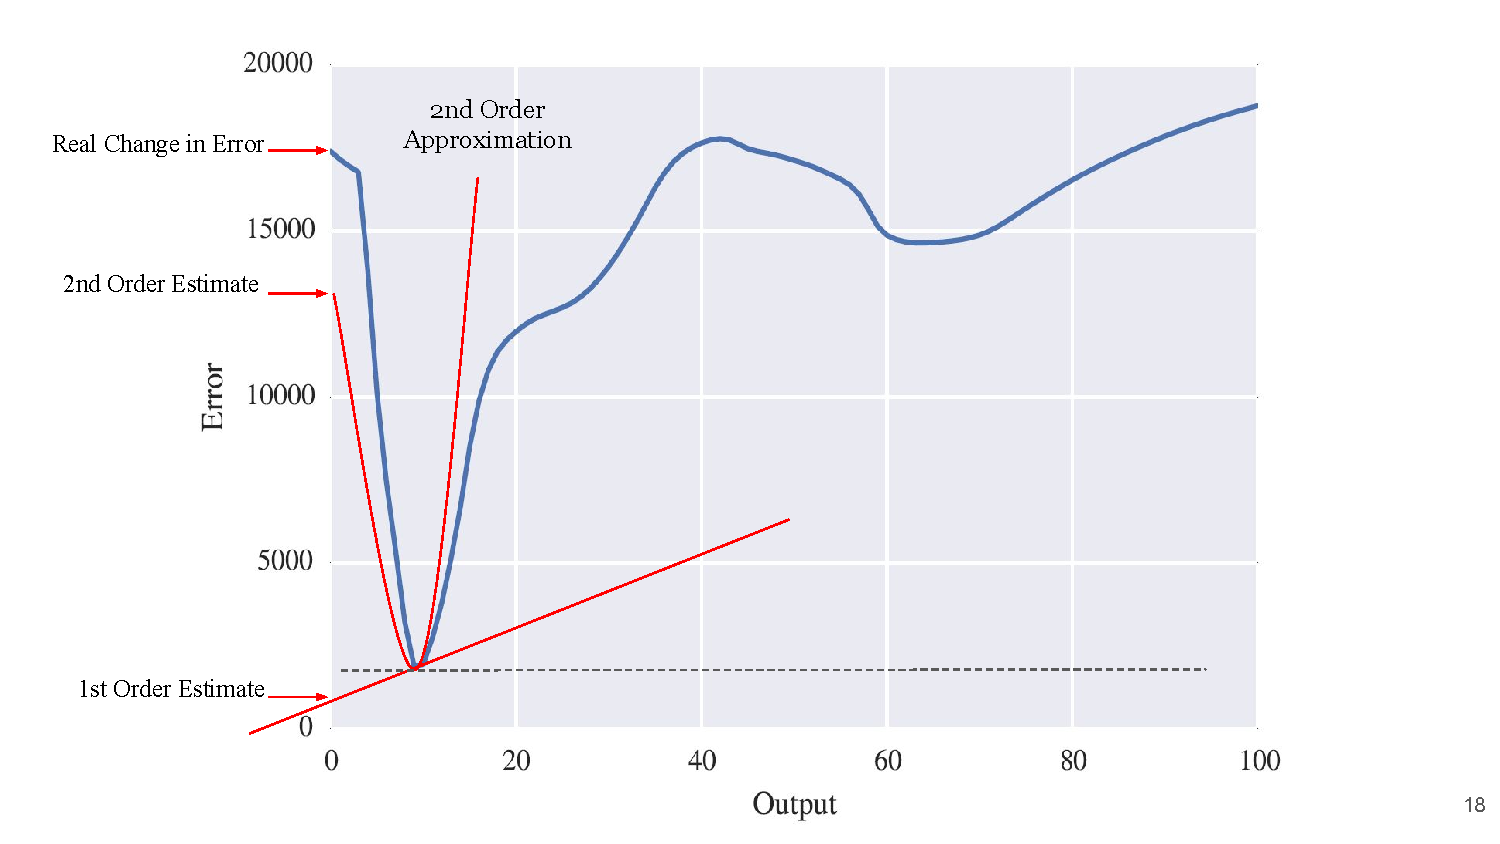
\includegraphics[width=\linewidth]{intuition.pdf}
  \caption{The intuition behind 1st \& 2nd order neuron pruning decisions}
  \label{fig:intuition}
\end{figure}

Figure \ref{fig:intuition} shows a random error function plotted against the output of any given neuron. Note that this figure is for illustration purposes only. The error function is minimized at a particular value of the neuron output as can be seen in the figure. The process of training a neural network is essentially the process of finding these minimizing output values for all the neurons in the network. Pruning this particular neuron (which translates to getting a zero output from it will result in a change in the total overall error. This change in error is represented by distance between the original minimum error (shown by the dashed line) and the top red arrow. This neuron is clearly a bad candidate for removal since removing it will result in a huge error increase. 

The straight red line in the figure represents the first-order approximation of the error using Taylor Series as described before while the parabola represents a second-order approximation. It can be clearly seen that the second-order approximation is a much better estimate of the change in error.

One thing to note here is that it is possible in some cases that there is some thresholding required when trying to approximate the error using the 2nd order Taylor Series expansion. These cases might arise when the parabolic approximation undergoes a steep slope change. To take into account such cases, mean and median thresholding were employed, where any change above a certain threshold was assigned a mean or median value respectively.

Two pruning algorithms are proposed here. They are different in the way the neurons are ranked but both of them use $\Delta E_{k}$, the approximation of the change in error as the basis for the ranking. $\Delta E_{k}$ can be calculated using the Brute Force method, or one of the two Taylor Series approximations discussed previously.

The first step in both the algorithms is to  decide a stopping criterion. This can vary depending on the application but some intuitive stopping criteria can be: maximum number of neurons to remove, percentage scaling needed, maximum allowable accuracy drop etc. 

\subsubsection{Algorithm I: Single Overall Ranking}
The complete algorithm is shown in Algorithm \ref{algo1}. The idea here is to generate a single ranked list based on the values of $\Delta E_{k}$. This involves a single pass of second-order back-propagation (without weight updates) to collect the gradients for each neuron. The neurons from this rank-list (with the lowest values of $\Delta E_{k}$) are then pruned according to the stopping criterion decided. We note here that this algorithm is intentionally naive and is used for comparison only. 

\begin{algorithm}
 \KwData{optimally trained network, training set}
 \KwResult{A pruned network}
 initialize and define stopping criterion \;
 
 perform forward propagation over the training set \;
 
  perform second-order back-propagation without updating weights and collect linear and quadratic gradients \;
  
  rank the remaining neurons based on $\Delta E_{k}$\;
  
 \While{stopping criterion is not met}{
  remove the last ranked neuron \;
  
 }
 \caption{Single Overall Ranking}
 \label{algo1}
\end{algorithm}
 
\subsubsection{Algorithm II: Iterative Re-Ranking}

In this greedy variation of the algorithm (Algorithm \ref{algo2}), after each neuron removal, the remaining network undergoes a single forward and backward pass of second-order back-propagation (without weight updates) and the rank list is formed again. Hence, each removal involves a new pass through the network. This method is computationally more expensive but takes into account the dependencies the neurons might have on one another which would lead to a change in error contribution every time a dependent neuron is removed. 

\begin{algorithm}
 \KwData{optimally trained network, training set}
 \KwResult{A pruned network}
 initialize and define stopping criterion \;
 
 \While{stopping criterion is not met}{
  perform forward propagation over the training set \;
  
  perform second-order back-propagation without updating weights and collect linear and quadratic gradients \;
  
  rank the remaining neurons based on $\Delta E_{k}$  \;
  
  
  remove the worst neuron based on the ranking \;
  
 }
 \caption{Iterative Re-Ranking}
 \label{algo2}
\end{algorithm}

\section{Experimental Results}
\subsection{Example Regression Problem}
This problem serves as a quick example to demonstrate many of the phenomena described in previous sections. We trained two networks to learn the cosine function, with one input and one output. This is a task which requires no more than 11 sigmoid neurons to solve entirely, and in this case we don't care about overfitting because the cosine function has a precise definition. Furthermore, the cosine function is a good toy example because it is a smooth continuous function and, as demonstrated by \cite{nielsen2015neural}, if we were to tinker directly with the weights and bias parameters of the network, we could allocate individual units within the network to be responsible for constrained ranges of inputs, similar to a basis spline function with many control points. This would distribute the learned function approximation evenly across all hidden units, and thus we have presented the network with a problem in which it could productively use as many hidden units as we give it. In this case, a pruning algorithm would observe a fairly consistent increase in error after the removal of each successive unit. In practice however, regardless of the number of experimental trials, this is not what happens. The network will always use 10-11 hidden units and leave the rest to cancel each other's influence.

\begin{figure}[!h]
\centering
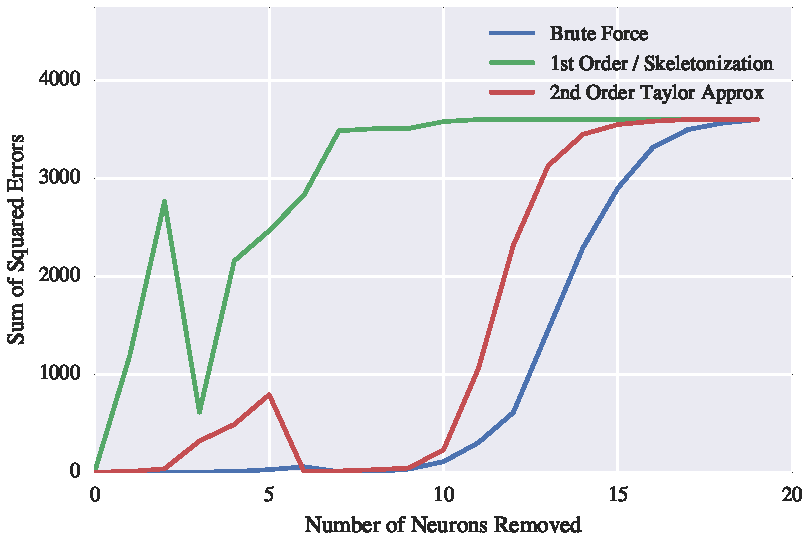
\includegraphics[width=0.49\linewidth]{png/cos-small.pdf}
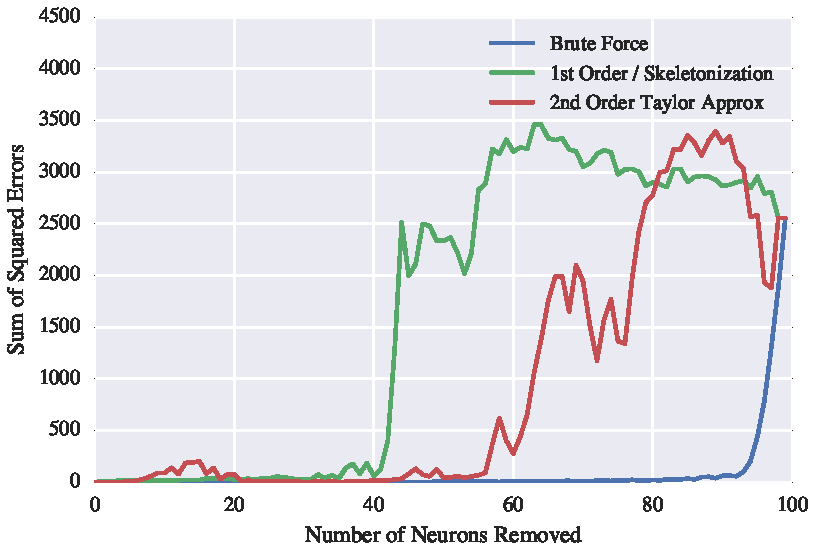
\includegraphics[width=0.49\linewidth]{png/cos-big.pdf}
\caption{Degradation in squared error after pruning a two-layer network trained to compute the cosine function (\textbf{Left Network:} 2 layers, 10 neurons each, 1 output, logistic sigmoid activation, starting test accuracy: 0.9999993, \textbf{Right Network:} 2 layers, 50 neurons each, 1 output, logistic sigmoid activation, starting test accuracy: 0.9999996)}
\label{fig:cosine-double-layer}
\end{figure}

Figure \ref{fig:cosine-double-layer} shows two graphs. Both graphs demonstrate the use of the iterative re-ranking algorithm and the comparative performance of the brute-force pruning method (in blue), the first order method (in green), and the second order method (in red). The graph on the left shows the performance of these algorithms starting from a network with two layers of 10 neurons (20 total), and the graph on the right shows a network with two layers of 50 neurons (100 total). 

In the left graph, we see that the brute-force method shows a graceful degradation, and the error only begins to rise sharply after 50\% of the total neurons have been removed. The error is basically constant up to that point. In the first and second order methods, we see evidence of poor decision making in the sense that both made mistakes early on, which disrupted the output function approximation. The first order method made a large error early on, though we see after a few more neurons were removed this error was corrected somewhat (though it only got worse from there). This is direct evidence of the lack of fault tolerance in a trained neural network. This phenomenon is even more starkly demonstrated in the second order method. After making a few poor neuron removal decisions in a row, the error signal rose sharply, and then went back to zero after the 6th neuron was removed. This is due to the fact that the neurons it chose to remove were trained to cancel each others' influence within a localized part of the network. After the entire group was eliminated, the approximation returned to normal. This can only happen if the output function approximation is not evenly distributed over the hidden units in a trained network. 

This phenomenon is even more starkly demonstrated in the graph on the right. Here we see the first order method got ``lucky'' in the beginning and made decent decisions up to about the 40th removed neuron. The second order method had a small error in the beginning which it recovered from gracefully and proceeded to pass the 50 neuron point before finally beginning to unravel. The brute force method, in sharp contrast, shows little to no increase in error at all until 90\% of the neurons in the network have been obliterated. Clearly first and second order methods have some value in that they do not make completely arbitrary choices, but the brute force method is far better at this task. 

This also demonstrates the sharp dualism in neuron roles within a trained network. These networks were trained to near-perfect precision and each pruning method was applied \textit{without} any re-training of any kind. Clearly, in the case of the brute force or oracle method, up to 90\% of the network can be completely extirpated before the output approximation even begins to show any signs of degradation. This would be impossible if the learning representation were evenly or equitably distributed. Note, for example, that the degradation point in both cases is approximately the same. This example is not a real-world application of course, but it brings into very clear focus the kind of phenomena we will discuss in the following sections. 

\subsection{Results on MNIST Dataset}
For all the results presented in this section, the MNIST database of Handwritten Digits by \cite{lecun-mnisthandwrittendigit-2010} was used. It is worth noting that due to the time taken by the brute force algorithm we rather used a 5000 image subset of the MNIST database in which we have normalized the pixel values between 0 and 1.0, and compressed the image sizes to 20x20 images rather than 28x28, so the starting test accuracy reported here appears higher than those reported by LeCun et al. We do not believe that this affects the interpretation of the presented results because the basic learning problem does not change with a larger dataset or input dimension.

\subsection{Pruning a 1-Layer Network}
The network architecture in this case consisted of 1 layer, 100 neurons, 10 outputs, logistic sigmoid activations, and a starting test accuracy of 0.998.

\subsubsection{Single Overall Ranking Algorithm}
We first present the results for a single-layer neural network in Figure \ref{fig:mnist-single-ranking-single-layer}, using the Single Overall algorithm (Algorithm \ref{algo1}) as proposed in Section \ref{sec2}. (We again note that this algorithm is intentionally naive and is used for comparison only. Its performance should be expected to be poor.) After training, each neuron is assigned its permanent ranking based on the three criteria discussed previously: A brute force ``ground truth'' ranking, and two approximations of this ranking using first and second order Taylor estimations of the change in network output error resulting from the removal of each neuron. 

\begin{figure}[!h]
\centering
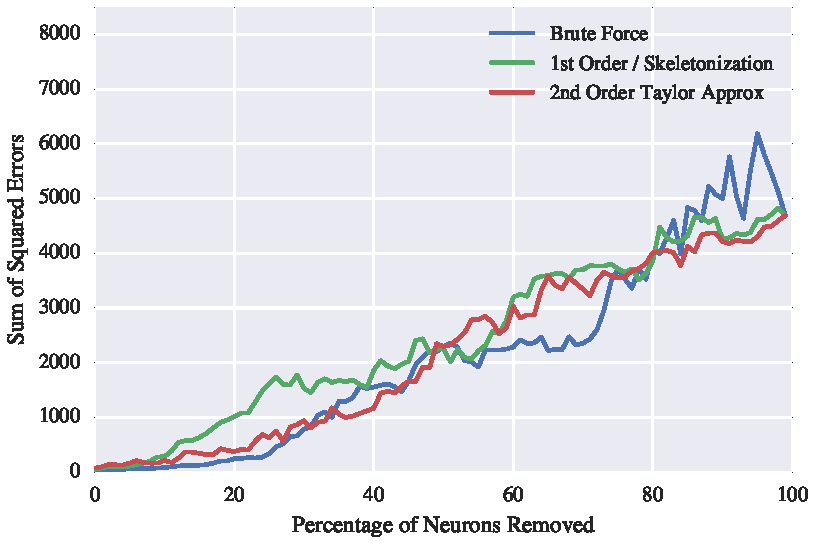
\includegraphics[width=0.49\linewidth]{png/mnist-acc99-single-pass-method.pdf}
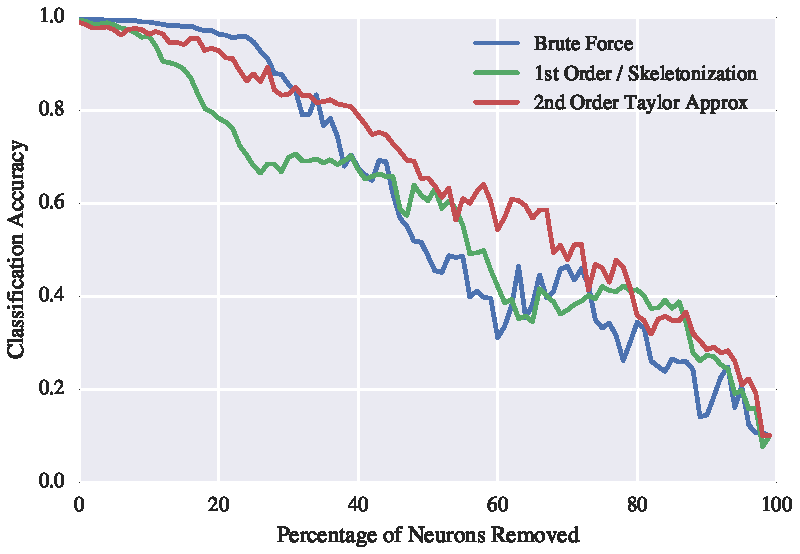
\includegraphics[width=0.49\linewidth]{png/mnist-acc99-single-pass-accuracy.pdf}
\caption{Degradation in squared error (left) and classification accuracy (right) after pruning a single-layer network using The Single Overall Ranking algorithm (\textbf{Network:} 1 layer, 100 neurons, 10 outputs, logistic sigmoid activation, starting test accuracy: 0.998)}
\label{fig:mnist-single-ranking-single-layer}
\end{figure}

An interesting observation here is that with only a single layer, no criteria for ranking the neurons in the network (brute force or the two Taylor Series variants) using Algorithm \ref{algo1} emerges superior, indicating that the 1st and 2nd order Taylor Series methods are actually reasonable approximations of the brute force method under certain conditions. Of course, this method is still quite bad in terms of the rate of degradation of the classification accuracy and in practice we would likely follow Algorithm \ref{algo2} which is takes into account \cite{mozer1989skeletonization}'s observations stated in the Related Work section. The purpose of the present investigation, however, is to demonstrate how much of a trained network can be theoretically removed without altering the network's learned parameters in any way.

\subsubsection{Iterative Re-Ranking Algorithm}

\begin{figure}[!hb]
\centering
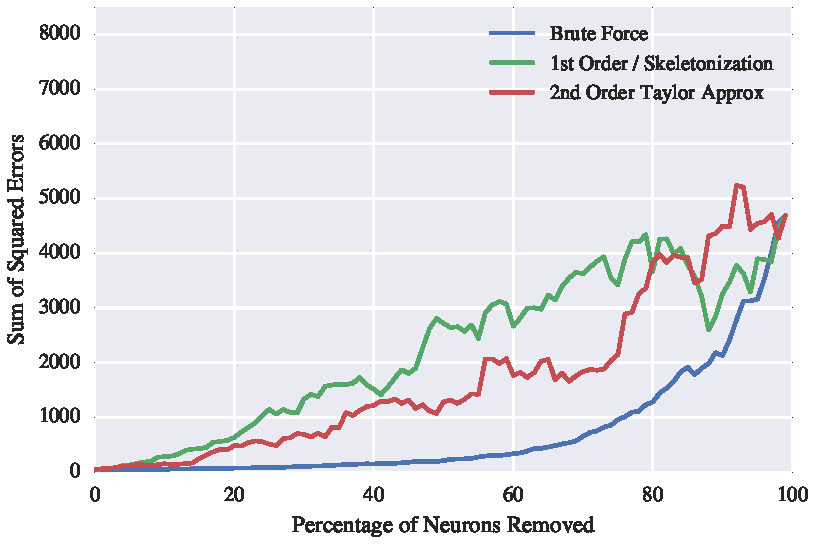
\includegraphics[width=0.49\linewidth]{png/mnist-acc99-iterative-rerank-method.pdf}
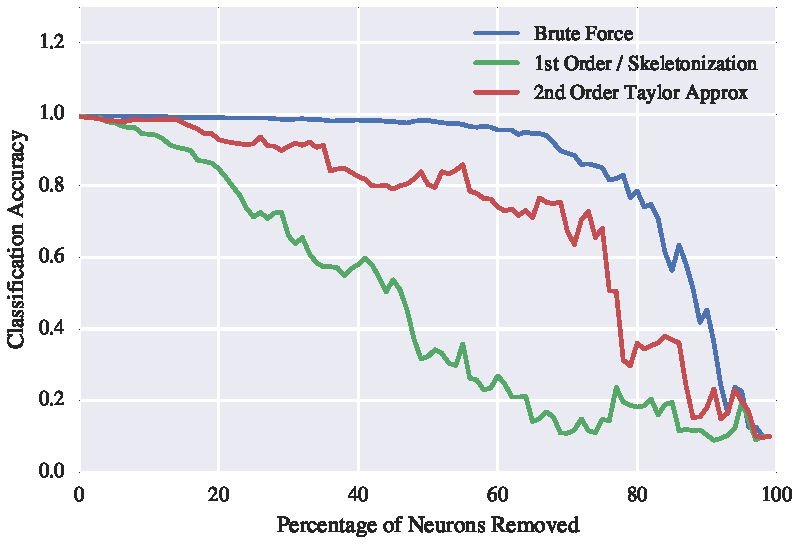
\includegraphics[width=0.49\linewidth]{png/mnist-acc99-iterative-rerank-accuracy.pdf}
\caption{Degradation in squared error (left) and classification accuracy (right) after pruning a single-layer network the Iterative Re-ranking algorithm (\textbf{Network:} 1 layer, 100 neurons, 10 outputs, logistic sigmoid activation, starting test accuracy: 0.998)}
\label{fig:mnist-re-ranking-single-layer}
\end{figure}

In Figure \ref{fig:mnist-re-ranking-single-layer} we present our results using Algorithm \ref{algo2} (The Iterative Re-Ranking Algorithm) in which all remaining neurons are re-ranked after each successive neuron is switched off. We compute the same brute force rankings and Taylor series approximations of error deltas over the remaining active neurons in the network after each pruning decision. This is intended to account for the effects of cancelling interactions between neurons. 

There are 2 key observations here. Using the Brute Force ranking criteria, almost 60\% of the neurons in the network can be pruned away without any major loss in performance. The other noteworthy observation here is that the 2nd order Taylor Series approximation of the error performs consistently better than its 1st order version.

%tl;dr: 1 layer is grrrreat for brute force! Clearly 2nd order method is consistently better than 1st order method. 

%tl;dr: Brute force method is amazing here! 1 layer makes things a lot easier, and a 2nd order method can do okay as well, but can still be improved a lot. 60% of neurons doing nothing!

\subsubsection{Visualization of Error Surface \& Pruning Decisions}

\begin{figure}[!hb]
\centering
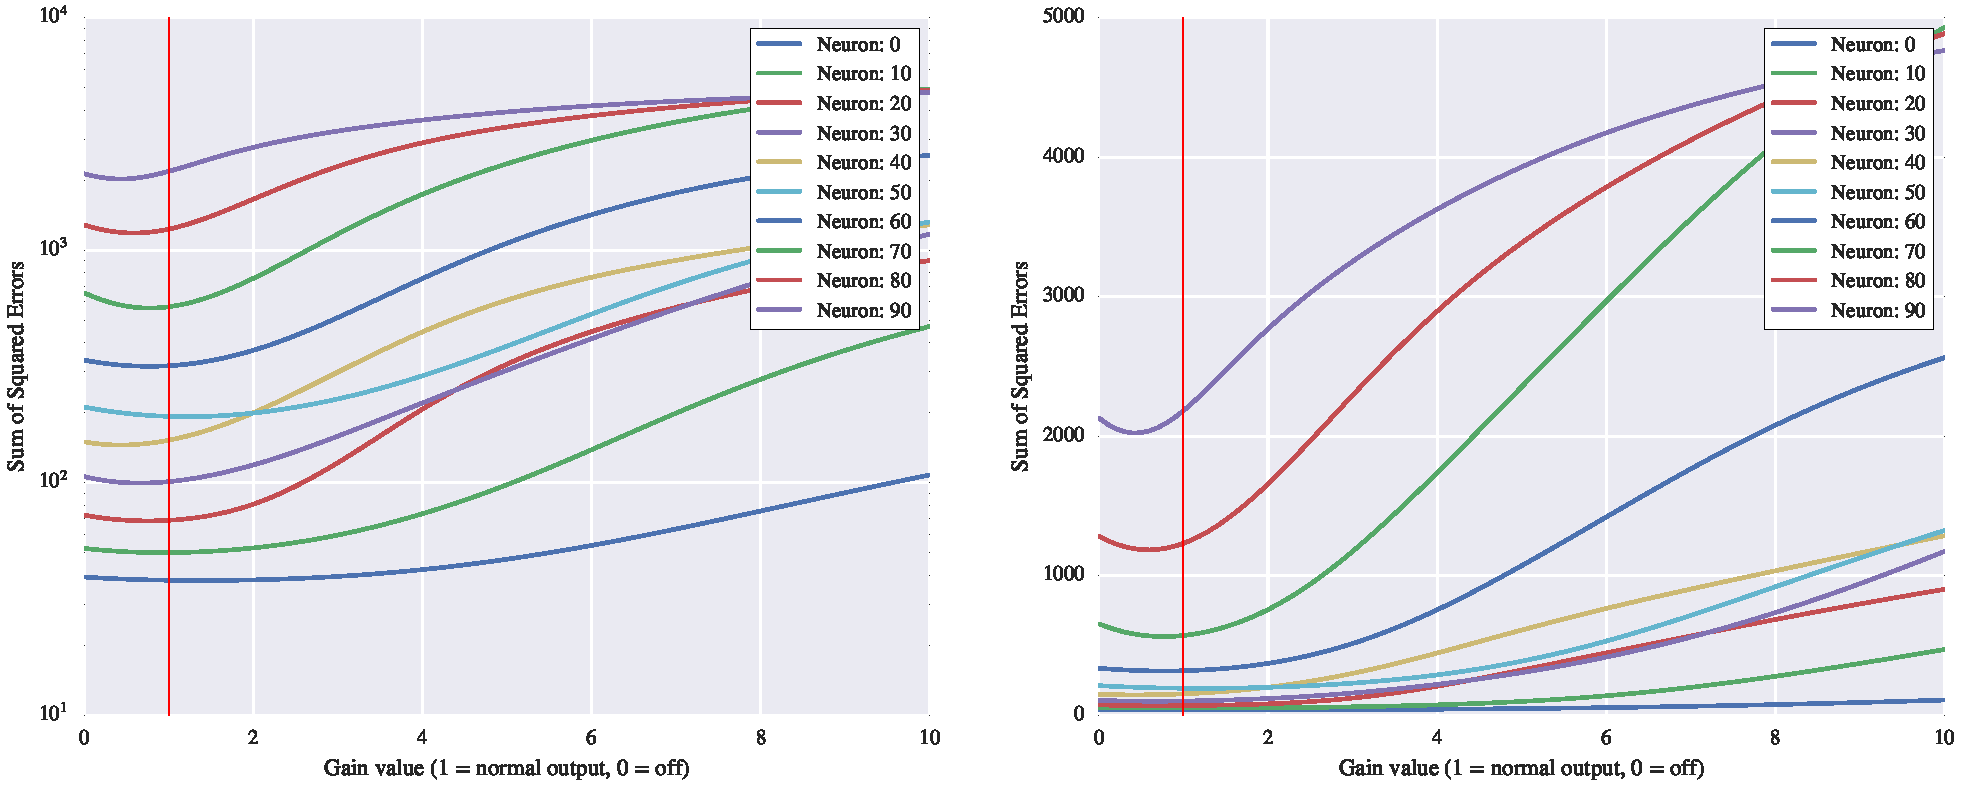
\includegraphics[width=\linewidth]{png/mnist-acc99-gt-gain.pdf}
\caption{Error surface of the network output in log space (left) and in real space (right) with respect to each candidate neuron chosen for removal using the brute force criterion; (\textbf{Network:} 1 layer, 100 neurons, 10 outputs, logistic sigmoid activation, starting test accuracy: 0.998)}
\label{fig:mnist-gt-single-layer}
\end{figure}

\begin{figure}[!hb]
\centering
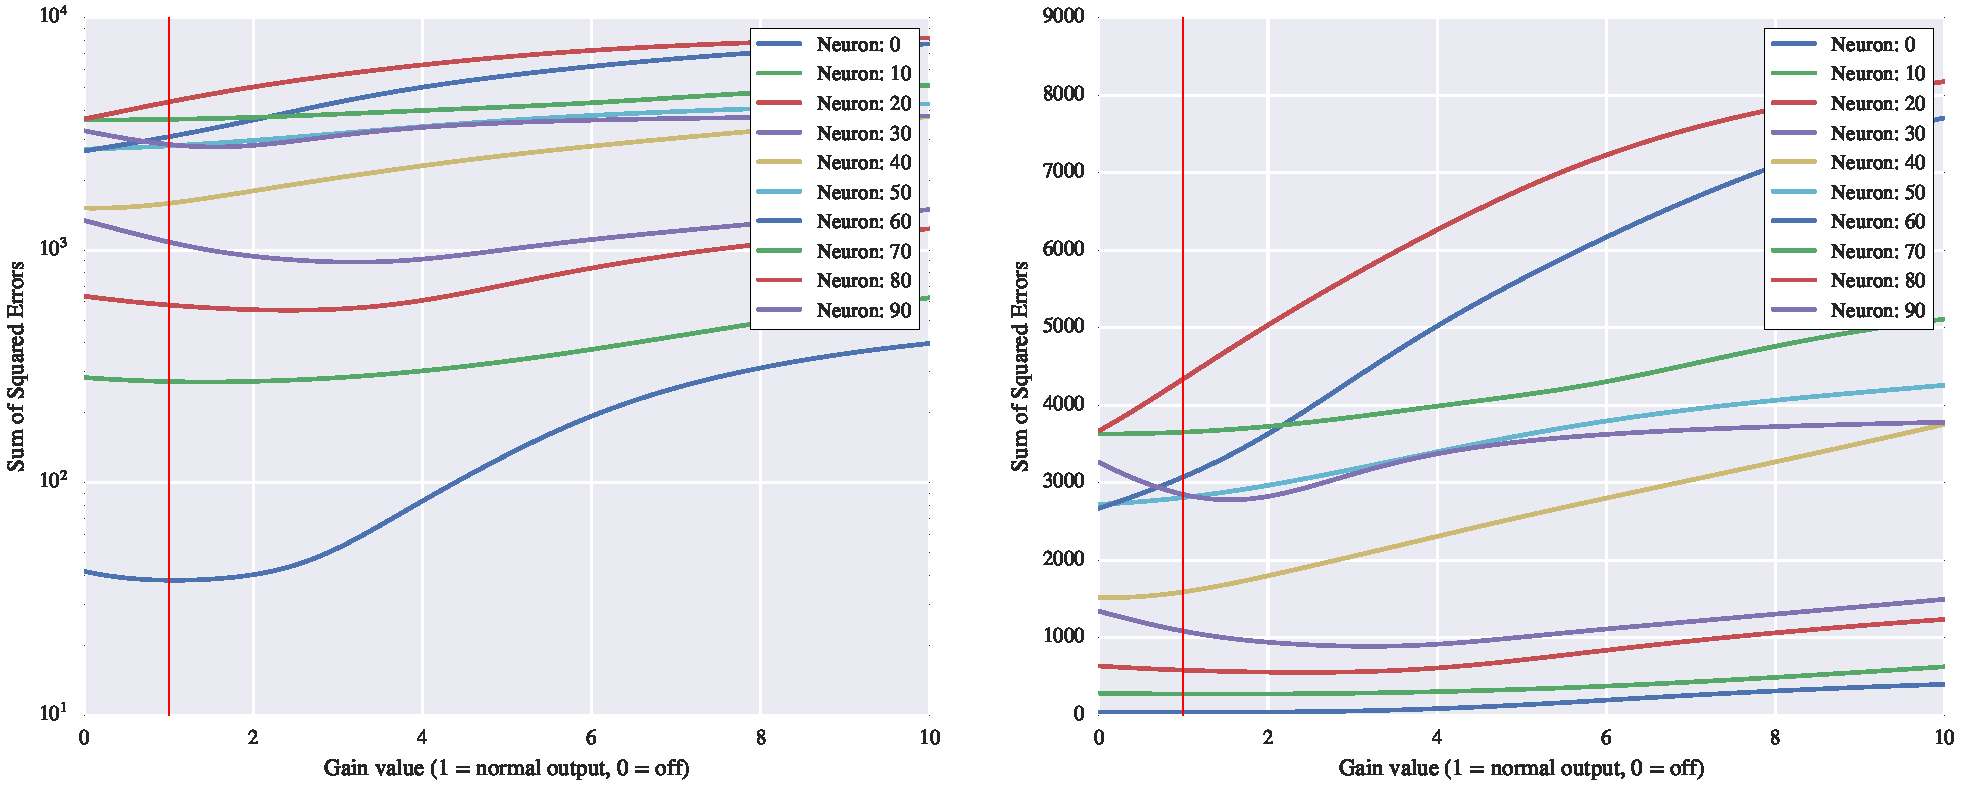
\includegraphics[width=\linewidth]{png/mnist-acc99-g1-gain.pdf}
\caption{Error surface of the network output in log space (left) and in real space (right) with respect to each candidate neuron chosen for removal using the 1st order Taylor Series error approximation criterion; (\textbf{Network:} 1 layer, 100 neurons, 10 outputs, logistic sigmoid activation, starting test accuracy: 0.998)}
\label{fig:mnist-gt-single-layer}
\end{figure}

\begin{figure}[!hb]
\centering
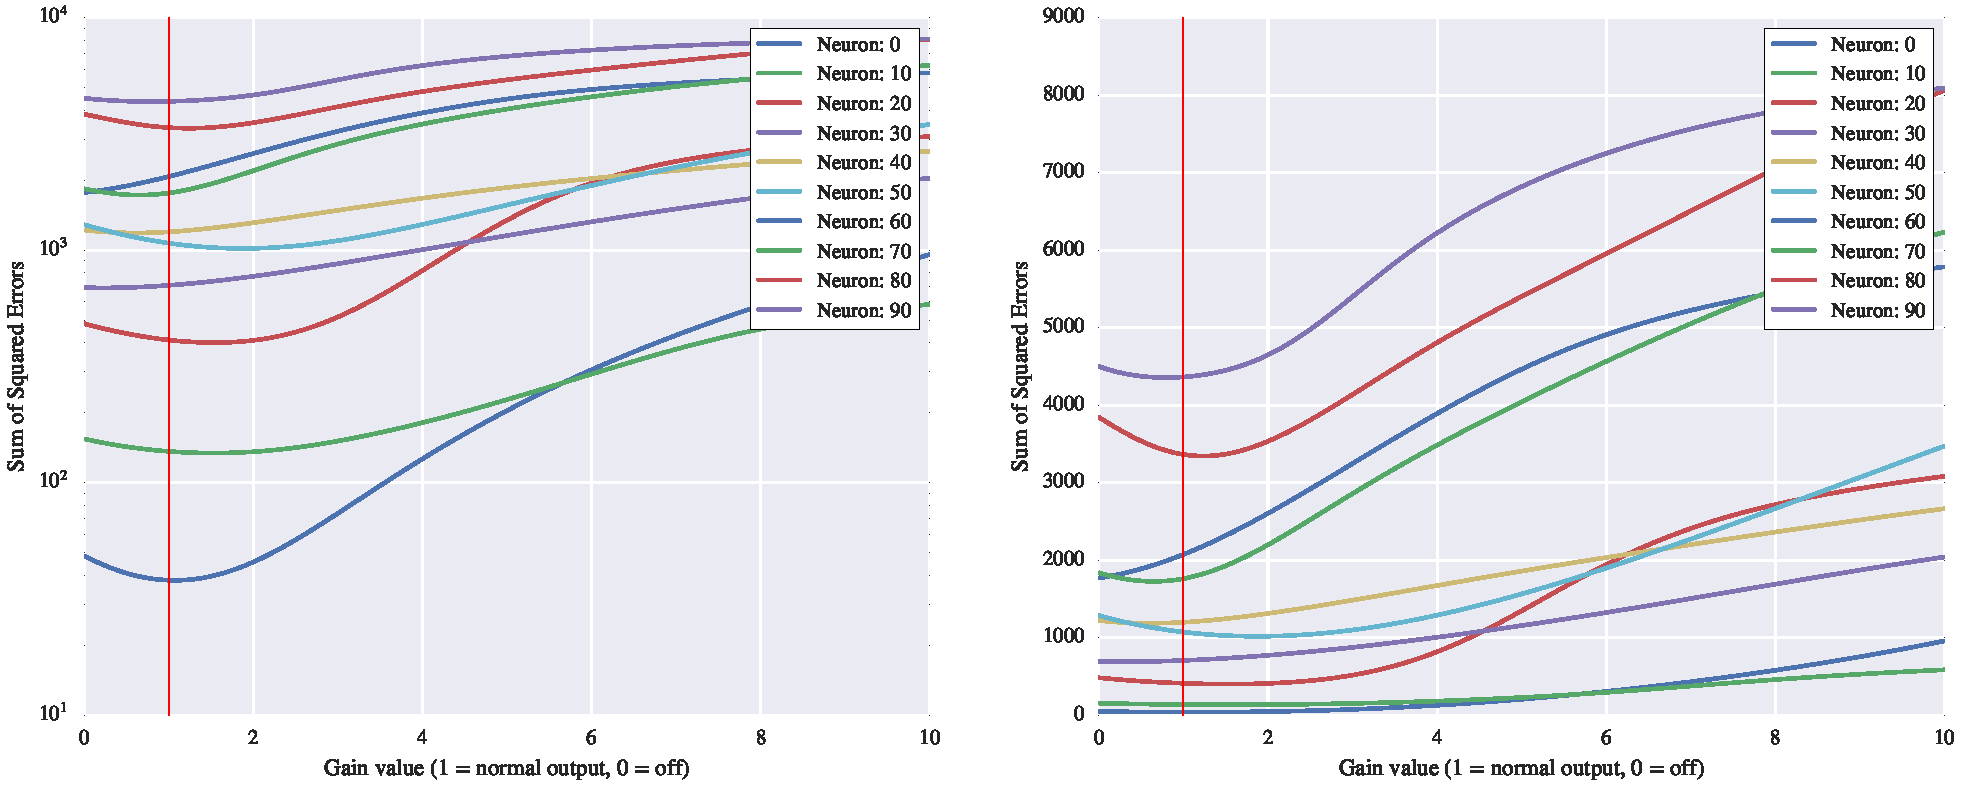
\includegraphics[width=\linewidth]{png/mnist-acc99-g2-gain.pdf}
\caption{Error surface of the network output in log space (left) and in real space (right) with respect to each candidate neuron chosen for removal using the 2nd order Taylor Series error approximation criterion; (\textbf{Network:} 1 layer, 100 neurons, 10 outputs, logistic sigmoid activation, starting test accuracy: 0.998)}
\label{fig:mnist-gt-single-layer}
\end{figure}

As explained in Section \ref{sec2}, these graphs are a visualization of the error surface of the network output with respect to the neurons chosen for removal using each of the 3 ranking criteria, represented in intervals of 10 neurons. In each graph, the error surface of the network output is displayed in log space (left) and in real space (right) with respect to each candidate neuron chosen for removal. We create these plots during the pruning exercise by picking a neuron to switch off, and then multiplying its output by a scalar gain value $\alpha$ which is adjusted from 0.0 to 10.0 with a step size of 0.001. When the value of $\alpha$ is 1.0, this represents the unperturbed neuron output learned during training. Between 0.0 and 1.0, we are graphing the literal effect of turning the neuron off ($\alpha = 0$), and when $\alpha > 1.0$ we are simulating a boosting of the neuron's influence in the network, i.e. inflating the value of its outgoing weight parameters. 

We graph the effect of boosting the neuron's output to demonstrate that for certain neurons in the network, even doubling, tripling, or quadrupling the scalar output of the neuron has no effect on the overall error of the network, indicating the remarkable degree to which the network has learned to ignore the value of certain parameters. In other cases, we can get a sense of the sensitivity of the network's output to the value of a given neuron when the curve rises steeply after the red 1.0 line. This indicates that the learned value of the parameters emanating from a given neuron are relatively important, and this is why we should ideally see sharper upticks in the curves for the later-removed neurons in the network, that is, when the neurons crucial to the learning representation start to be picked off. 

%Remember that lower is better in terms of the height of the curve and minimal horizontal change between the vertical red line at 1.0 (neuron \textit{on}, $\alpha = 1.0$) and 0.0 (neuron \textit{off}, $\alpha = 0.0$) is indicative of a good candidate neuron to prune, i.e. there will be minimal effect on the network output when the neuron is removed. 

Some very interesting observations can be made in each of these graphs.

\textbf{Brute Force Criterion}

Notice how low to the floor and flat most of these curves are. It's only until the 90th removed neuron that we see a higher curve with a more convex shape (clearly a more influential piece of the network). This again validates the fact that a good majority of the neurons in a network do not contribute to the overall performance. 

\textbf{1st Order Approximation Criterion}

It can be seen that most choices seem to have flat or negatively sloped curves, indicating that the first order approximation seems to be pretty good, but examining the brute force choices shows they could be better. 

\textbf{2nd Order Approximation Criterion}

This method looks much more similar to the Brute Force method choices, though clearly not as good (they're more spread out). Notice the difference in convexity between the 2nd and 1st order method choices. It's clear that the first order method is fitting a line and the 2nd order method is fitting a parabola in their approximation. 

\subsection{Pruning A 2-Layer Network}
The network architecture in this case consisted of 2 layers, 50 neurons per layer, 10 outputs, logistic sigmoid activations, and a starting test accuracy of 1.000.
\subsubsection{Single Overall Ranking Algorithm}

\begin{figure}[!hb]
\centering
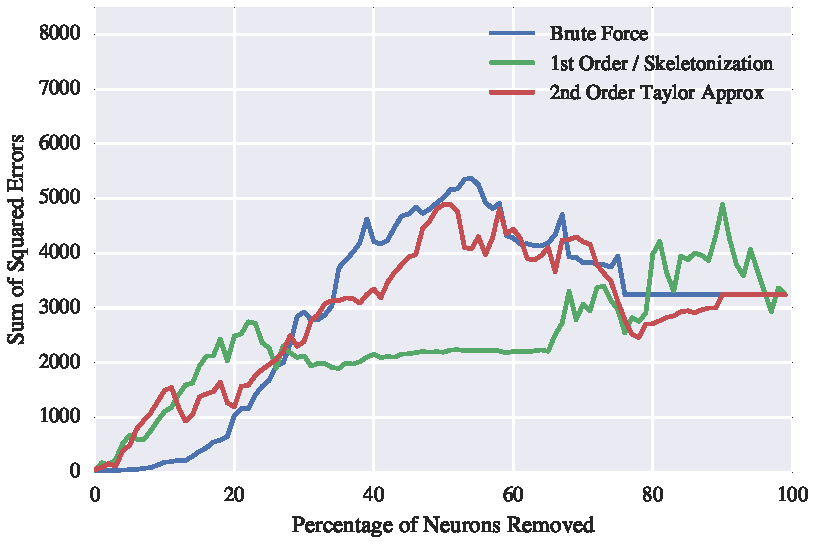
\includegraphics[width=0.49\linewidth]{png/mnist-deep-single-pass-method.pdf}
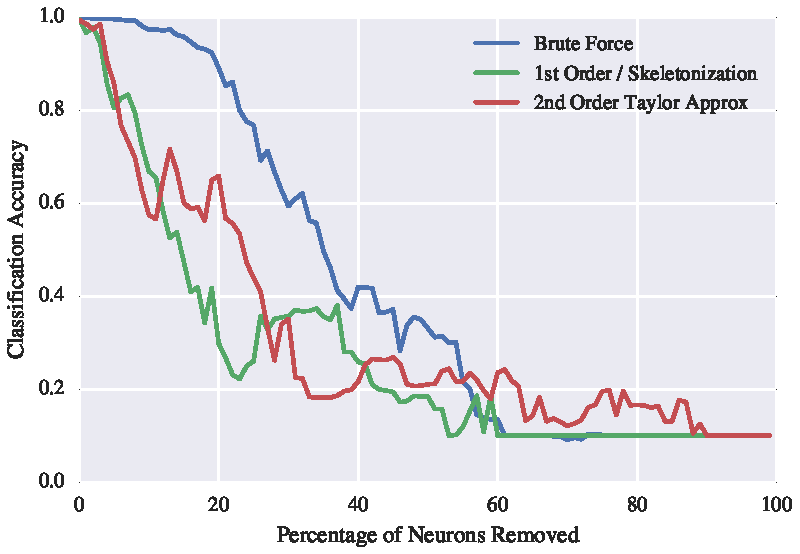
\includegraphics[width=0.49\linewidth]{png/mnist-deep-single-pass-accuracy.pdf}
\caption{Degradation in squared error (left) and classification accuracy (right) after pruning a 2-layer network using the Single Overall Ranking algorithm; (\textbf{Network:} 2 layers, 50 neurons/layer, 10 outputs, logistic sigmoid activation, starting test accuracy: 1.000)}
\label{fig:mnist-single-ranking-double-layer}
\end{figure}

Figure \ref{fig:mnist-single-ranking-double-layer} shows the pruning results for Algorithm \ref{algo1} on a 2-layer network. The ranking procedure is identical to the one used to generate Figure \ref{fig:mnist-single-ranking-single-layer}. (We again note that this algorithm is intentionally naive and is used for comparison only. Its performance should be expected to be poor.) 

Unsurprisingly, a 2-layer network is harder to prune because a single overall ranking will never capture the interdependencies between neurons in different layers. It makes sense that this is much worse than the performance on the 1-layer network, even if this method is already known to be bad, and we'd likely never use it in practice. 


\subsubsection{Iterative Re-Ranking Algorithm}

\begin{figure}[!hb]
\centering
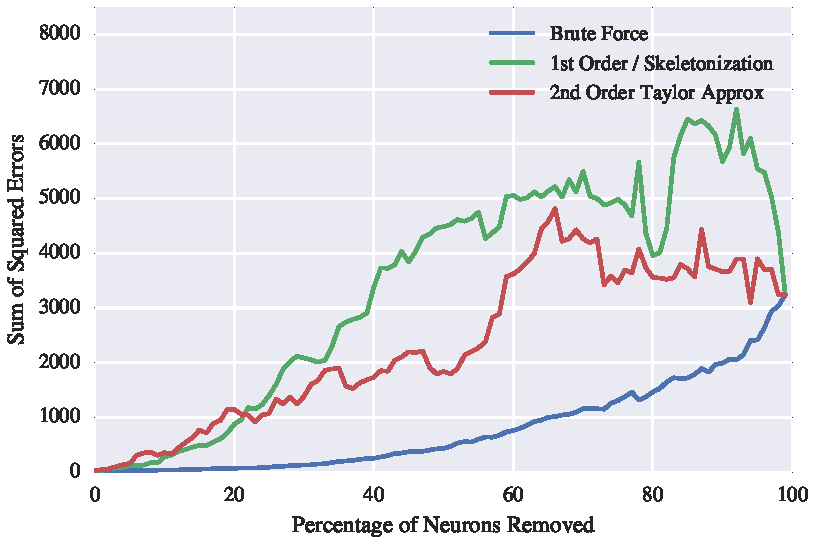
\includegraphics[width=0.49\linewidth]{png/mnist-deep-iterative-rerank-method.pdf}
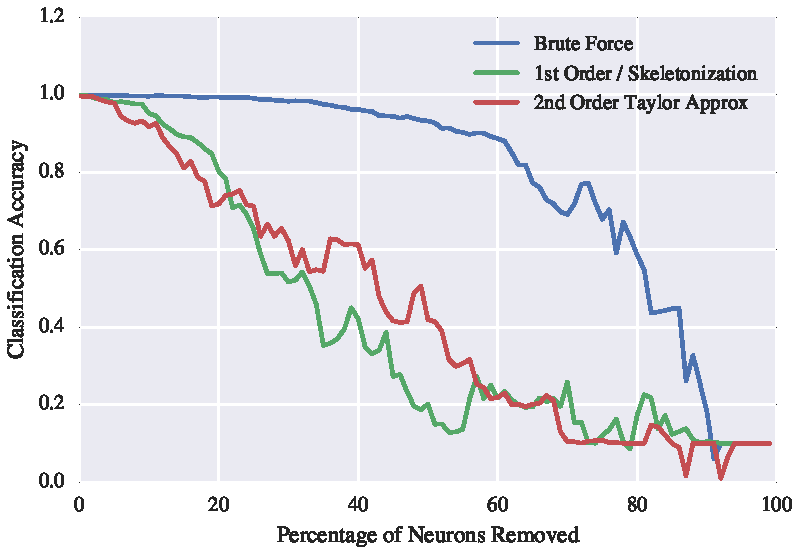
\includegraphics[width=0.49\linewidth]{png/mnist-deep-iterative-rerank-accuracy.pdf}
\caption{Degradation in squared error (left) and classification accuracy (right) after pruning a 2-layer network using the Iterative Re-ranking algorithm; (\textbf{Network:} 2 layers, 50 neurons/layer, 10 outputs, logistic sigmoid activation, starting test accuracy: 1.000)}
\label{fig:mnist-re-ranking-double-layer}
\end{figure}

Figure \ref{fig:mnist-re-ranking-double-layer} shows the results from using Algorithm \ref{algo2} on a 2-layer network. We compute the same brute force rankings and Taylor series approximations of error deltas over the remaining active neurons in the network after each pruning decision used to generate Figure \ref{fig:mnist-re-ranking-single-layer}. Again, this is intended to account for the effects of cancelling interactions between neurons. 

It is clear that it becomes harder to remove neurons 1-by-1 with a deeper network (which makes sense because the neurons have more interdependencies in a deeper network), but we see an overall better performance with 2nd order method vs. 1st order, except for the first 20\% of the neurons (but this doesn't seem to make much difference for classification accuracy.) 

Perhaps a more important observation here is that even with a more complex network, it is possible to remove up to 40\% of the neurons with no major loss in performance which is clearly illustrated by the brute force curve. This shows the clear potential of an ideal pruning technique and also shows how inconsistent 1st and 2nd order Taylor Series approximations of the error can be as ranking criteria.

\subsubsection{Visualization of Error Surface \& Pruning Decisions}

\begin{figure}[!hb]
\centering
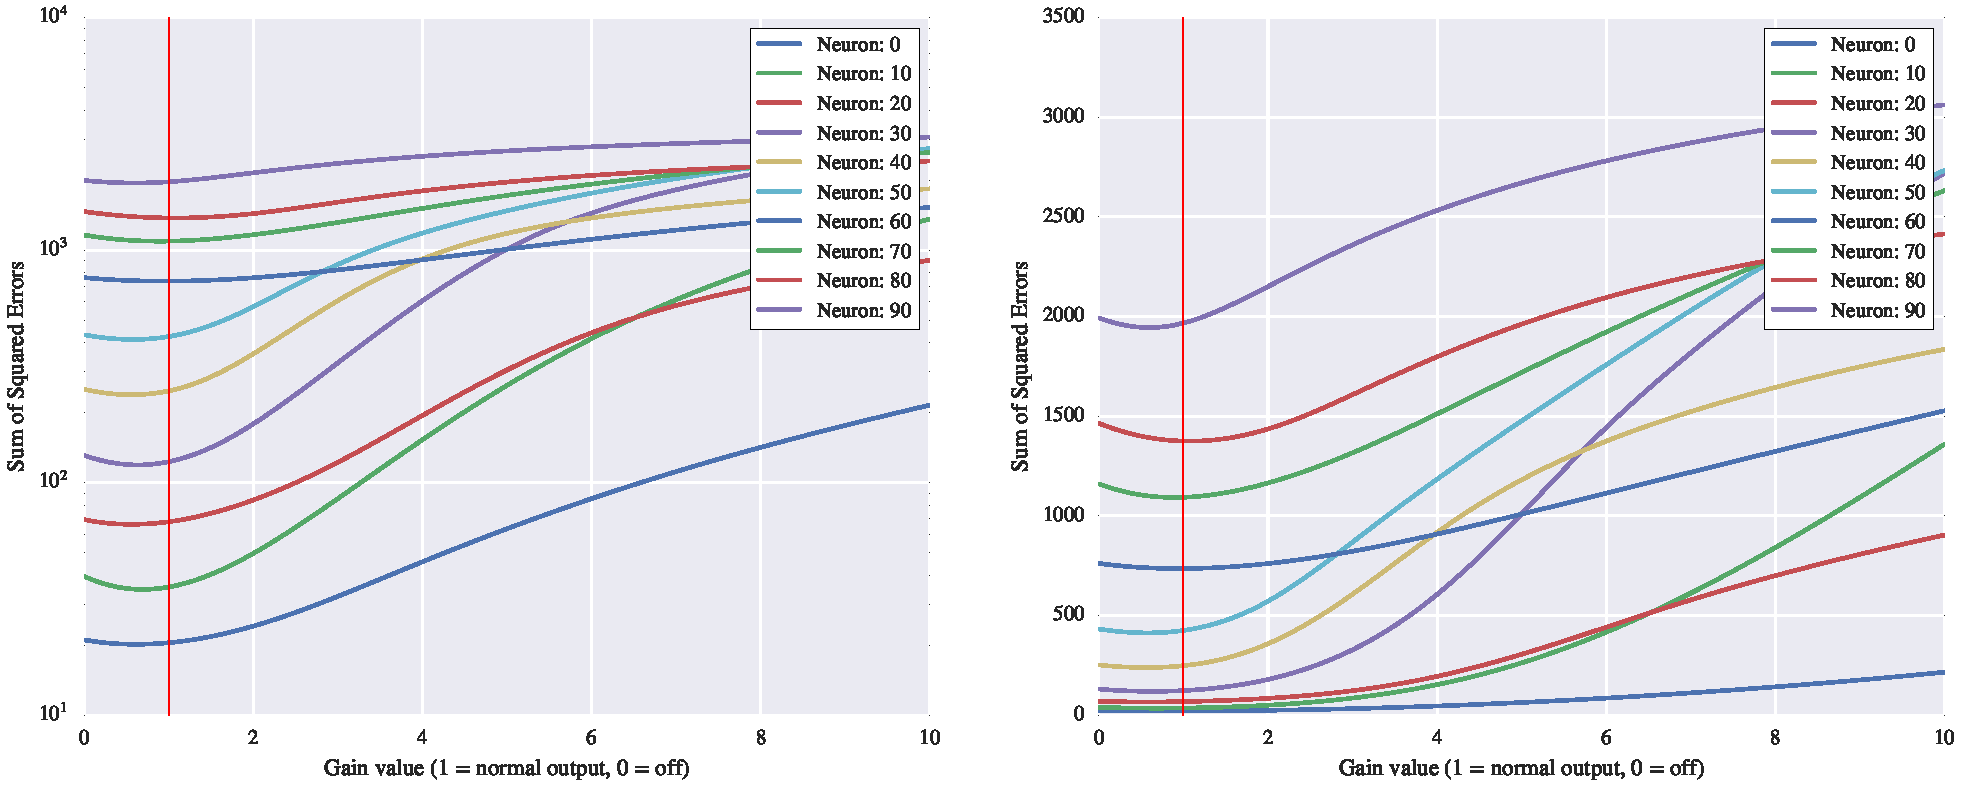
\includegraphics[width=\linewidth]{png/mnist-deep-gt-gain.pdf}
\caption{Error surface of the network output in log space (left) and in real space (right) with respect to each candidate neuron chosen for removal using the brute force criterion; (\textbf{Network:} 2 layers, 50 neurons/layer, 10 outputs, logistic sigmoid activation, starting test accuracy: 1.000)}
\label{fig:mnist-gt-double-layer}
\end{figure}

\begin{figure}[!hb]
\centering
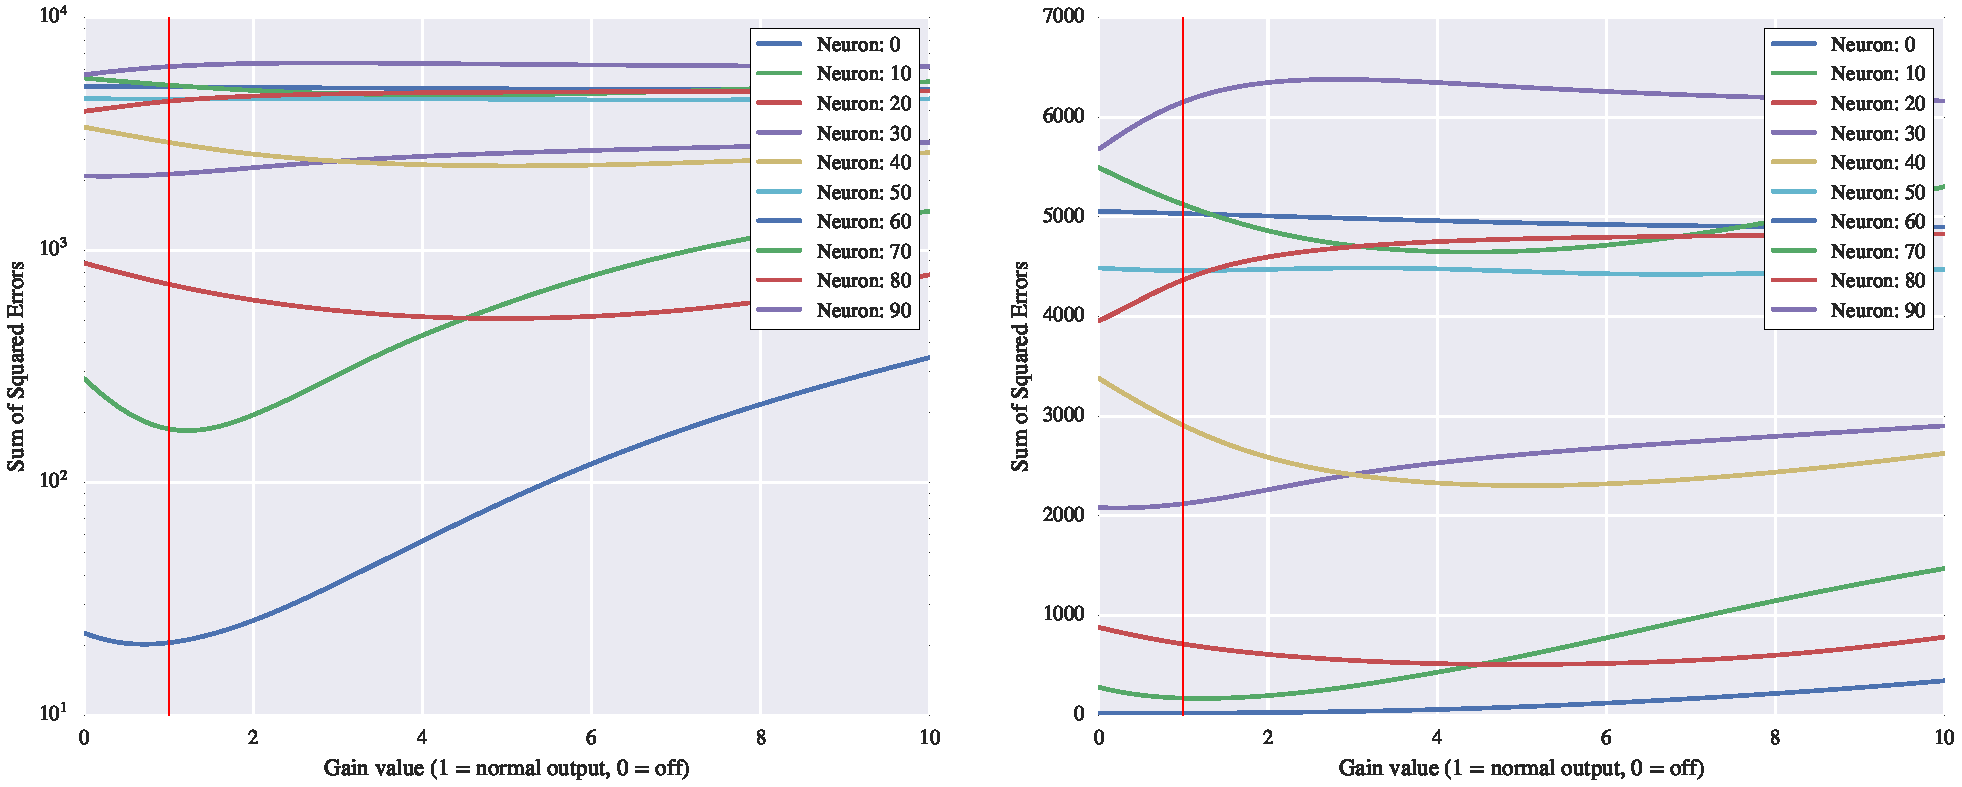
\includegraphics[width=\linewidth]{png/mnist-deep-g1-gain.pdf}
\caption{Error surface of the network output in log space (left) and in real space (right) with respect to each candidate neuron chosen for removal using the 1st order Taylor Series error approximation criterion; (\textbf{Network:} 2 layers, 50 neurons/layer, 10 outputs, logistic sigmoid activation, starting test accuracy: 1.000)}
\label{fig:mnist-g1-double-layer}
\end{figure}

\begin{figure}[!hb]
\centering
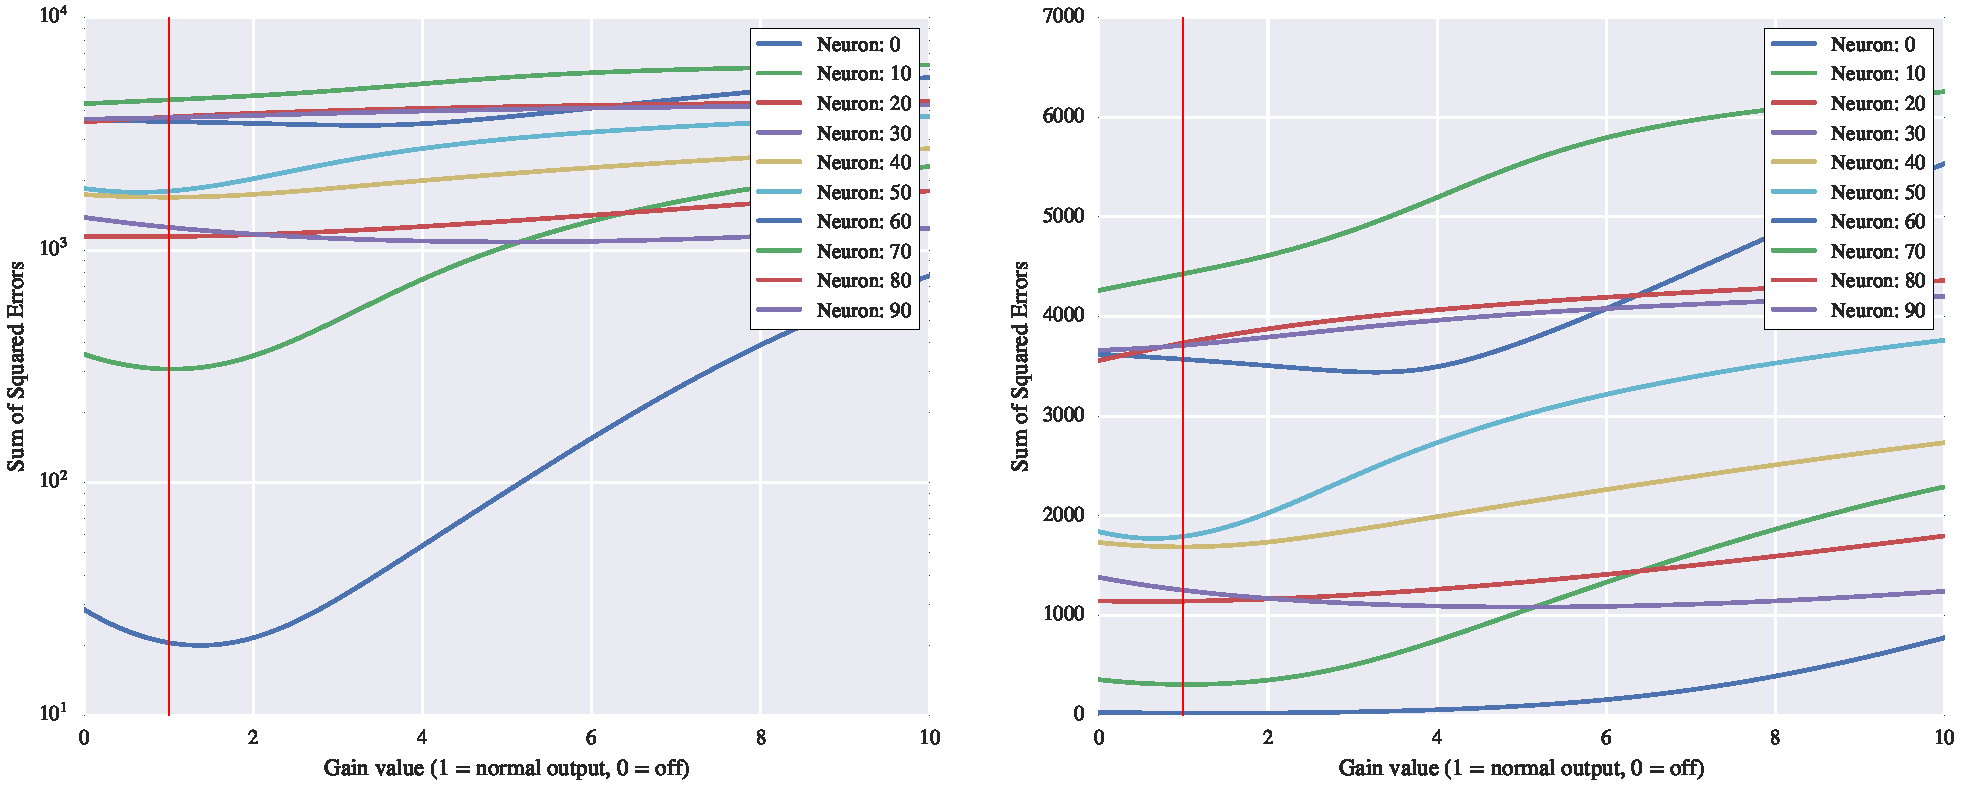
\includegraphics[width=\linewidth]{png/mnist-deep-g2-gain.pdf}
\caption{Error surface of the network output in log space (left) and in real space (right) with respect to each candidate neuron chosen for removal using the 2nd order Taylor Series error approximation criterion; (\textbf{Network:} 2 layers, 50 neurons/layer, 10 outputs, logistic sigmoid activation, starting test accuracy: 1.000)}
\label{fig:mnist-g2-double-layer}
\end{figure}


As seen in the case of a single layered network, these graphs are a visualization the error surface of the network output with respect to the neurons chosen for removal using each algorithm, represented in intervals of 10 neurons. 

\textbf{Brute Force Criterion}

It is clear why these neurons got chosen, their graphs clearly show little change when neuron is removed, are mostly near the floor, and show convex behaviour of error surface, which argues for the rationalization of using 2nd order methods to estimate difference in error when they are turned off.

\textbf{1st Order Approximation Criterion}

Drawing a flat line at the point of each neurons intersection with the red vertical line (no change in gain) shows that the 1st derivative method is actually accurate for estimation of change in error in these cases, but still ultimately leads to poor decisions. 

\textbf{2nd Order Approximation Criterion}

Clearly these neurons are not overtly poor candidates for removal (error doesn't change much between 1.0 \& zero-crossing left-hand-side), but could be better (as described above in the Brute Force Criterion discussion).


\subsection{Experiments on Toy Datasets}

\begin{figure}[!hb]
\centering
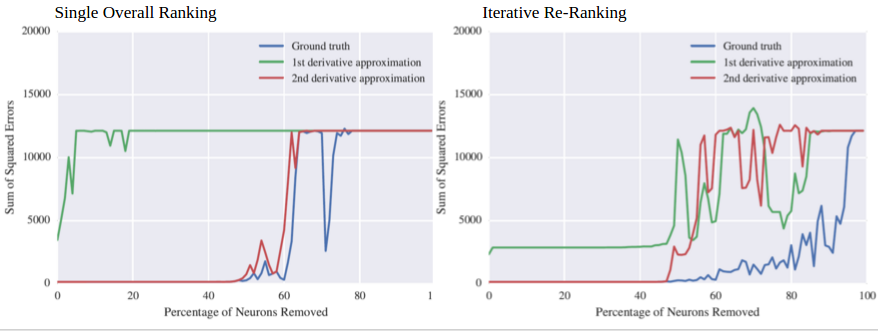
\includegraphics[width=0.80\linewidth]{png/diamond.png}
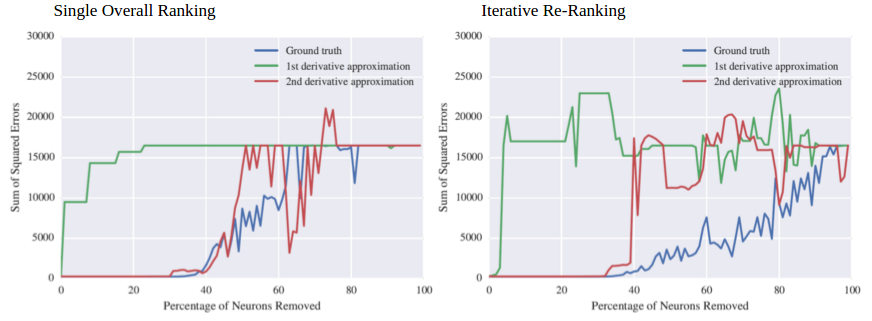
\includegraphics[width=0.80\linewidth]{png/rshape.png}
\caption{Degradation in squared error after pruning a 2-layer network using the Single Pass Algorithm (left) and the Iterative Re-ranking algorithm(right) on toy "diamond" shape dataset (above) and toy "random shape" dataset (below); (\textbf{Network:} 2 layers, 50 neurons/layer, 10 outputs, logistic sigmoid activation, starting test accuracy: 0.992(diamond); 0.986(random shape)}
\label{fig:diamond}
\end{figure}


As can be seen from the experiments on MNIST, even though the 2nd-order approximation criterion is consistently better than 1st-order, it's performance is not nearly as good as brute force based ranking, especially beyond the first layer. What is interesting to note is that from some other experiments conducted on toy datasets (predicting whether a given point would lie inside a given shape on the Cartesian plane), the performance of the 2nd-order method was found to be exceptionally good and produced results very close to the brute force method. The 1st-order method, as expected, performed poorly here as well. Some of these results are illustrated in Figure \ref{fig:diamond}. This huge variation in results from MNIST might be attributed to the fact that these toy datasets had only 2 output classes (as opposed to 10 classes in MNIST), but it certainly warrants further investigation.

%\begin{figure}[!hb]
%\centering
%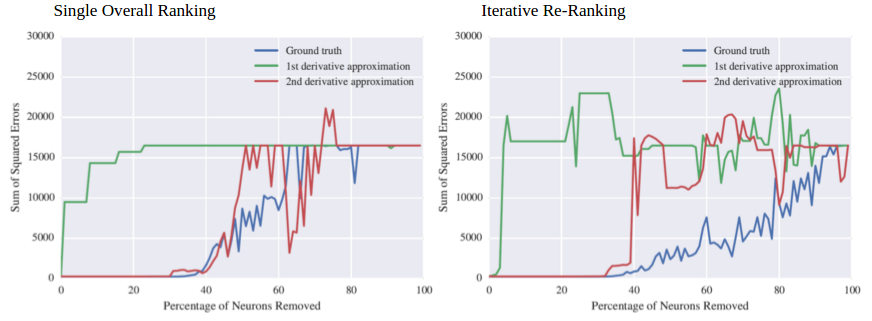
\includegraphics[width=0.80\linewidth]{png/rshape.png}
%\caption{Degradation in squared error after pruning a 2-layer network using the Single Pass Algorithm (left) and the Iterative Re-ranking algorithm(right) on toy "random shape" dataset; (\textbf{Network:} 2 layers, 50 neurons/layer, 10 outputs, logistic sigmoid activation, starting test accuracy: 0.986)}
%\label{fig:rshape}
%\end{figure}


%It was also observed that the brute force method primarily prunes neurons from the outer layer initially, which suggests that it might be a good idea to look into pruning neurons based on the layer they belong to.

%From some other experiments conducted on smaller toy datasets, it was noted that the pruning performance is worse if the models are not trained to a high accuracy, which is quite expected since this simply means that in these cases all the neurons have significant contribution to the network's performance and hence there is still scope for a better accuracy given more neurons and/or increased training times. However, pruning in these cases typically improved the MSE for the first 5 to 10 \% of neurons removed which can again be attributed to the theory put forward by \cite{mozer1989using}.
\section{Conclusions \& Future Work}
%\subsection{Conclusions}
Pruning neurons (instead of pruning individual weights) in a pre-trained neural network without seeing a major loss in performance is not only possible but also enables compressing networks to 40-80\% of their original size, which is of great importance in constrained memory environments like embedded devices. This fact is established through the experiments using the brute force criterion, which if made computationally viable (through parallelization) or approximated more efficiently than the Taylor Series based methods discussed in this paper, can prove to be a useful compression tool. It would also be interesting to see how these methods perform on deeper networks and on some other popular and real world datasets. Also, as mentioned in Section \ref{sec2}, we have not considered all possible combinations of neuron interdependence in this work due to the in-feasibility of implementation and have always pruned one neuron at a time. Even though the greedy evaluation of such combinations is highly prohibitive, it is not entirely implausible to think that algorithms can be developed for it in the future. That would help in truly tapping into the power of these interconnections and hopefully lead to impressive performance results.

The experiments on the visualization of error surfaces and pruning decisions concretely establish the fact that not all neurons in a network contribute to its performance in the same way. This confirms the idea put forth by \cite{mozer1989using} that learning representation is not distributed uniformly across neurons. Neural networks use a few neurons to learn the function approximation, and the remaining neurons cooperate to cancel out each other's effects. This is also a strong indication of the fact that once training is done, bigger networks do not hold an advantage over smaller ones, which is similar to the idea put forth by \cite{darkknowledge2015} in their work on ensemble learning techniques.

%It might also be interesting to see if the Cascade Correlation architecture arrives at the same number of final neurons as the pruning technique discussed in this paper.


\bibliography{iclr2017_conference}
\bibliographystyle{iclr2017_conference}

\newpage
\begin{center}
\appendix{APPENDIX}
\end{center}

\section{Second Derivative Back-Propagation}\label{apd:first}
\begin{figure}[bh!]
\centering
\newcommand{\repSigmoid}{$\sigma(\cdot)$}
\newcommand{\repLinear}{$\sum$}
\newcommand{\repMse}{MSE}
\newcommand{\repFirstSum}{$\Input j 1$}
\newcommand{\repLastSum}{$\Input i 0$}
\newcommand{\repFirstOutput}{\hspace{1.5cm}$\Con j i 0 \!=\! \Weight j i 0 \Out j 1$}
\newcommand{\repLastOutput}{$\Out i 0$}
\newcommand{\repLoss}{$E$}
\def\svgwidth{0.9\textwidth}
\hspace{-2cm}
\import{}{drawing.pdf_tex}
\hspace{-2cm}
\caption{A computational graph of a simple feed-forward network illustrating the naming of different variables, where $\sigma(\cdot)$ is the nonlinearity, MSE is the mean-squared error cost function and $E$ is the overall loss.}
\label{fig:comp_graph}
\end{figure}
%\pagebreak
%\section{Appendix A: Second Derivative Back-Propagation}
Name and network definitions:\\
\begin{align}
E &= \frac{1}{2}\sum\limits_i (\Out i 0 - \Target i)^2 &
\Out i m &= \sigma(\Input i m) &
\Input i m &= \sum\limits_j {\Weight j i m}{ \Out j {m + 1}} &
\Con j i m = \Weight j i m \Out j {m+1}
\end{align}
Superscripts represent the index of the layer of the network in question, with 0 representing the output layer. $E$ is the squared-error network cost function. $\Out i m$ is the $i$th output in layer $m$ generated by the activation function $\sigma$, which in this paper is is the standard logistic sigmoid. $\Input i m$ is the weighted sum of inputs to the $i$th neuron in the $m$th layer, and $\Con j i m$ is the contribution of the $j$th neuron in the $m+1$ layer to the input of the $i$th neuron in the $m$th layer. 
\subsection{First and Second Derivatives} 
The first and second derivatives of the cost function with respect to the outputs:
\begin{align}
\pdv{E}{\Out i 0} &= \Out i 0 - \Target i \label{cost_func_derivative}
\end{align}
\begin{align}
\pdv[2]{E}{{\Out i 0}} &= 1\label{cost_func_2nd_derivative}
\end{align}
The first and second derivatives of the sigmoid function in forms depending only on the output:
\begin{align}
\sigma^{\prime}(x) &= \sigma(x)\left(1 - \sigma(x)\right)\label{sigmoid_derivative} 
\\
\sigma^{\prime\prime}(x) &= \sigma^{\prime}(x)\left(1 - 2\sigma(x)\right) \label{sigmoid_2nd_derivative}
\end{align}
The second derivative of the sigmoid is easily derived from the first derivative:
\begin{align}
\sigma^{\prime}(x) &= \sigma(x)\left(1 - \sigma(x)\right)
\\
\sigma^{\prime\prime}(x) &= \dv{}{x}
\underbrace{\sigma(x)}_{f(x)}
\underbrace{\left(1 - \sigma(x)\right)}_{g(x)}
\\
\sigma^{\prime\prime}(x) &= f^{\prime}(x)g(x) + f(x)g^{\prime}(x)
\\
\sigma^{\prime\prime}(x) &= \sigma^{\prime}(x)(1-\sigma(x)) - \sigma(x)\sigma^{\prime}(x)
\\
\sigma^{\prime\prime}(x) &= \sigma^{\prime}(x) - 2\sigma(x)\sigma^{\prime}(x)
\\
\sigma^{\prime\prime}(x) &= \sigma^{\prime}(x)(1 - 2\sigma(x))
\end{align}

And for future convenience: 
\begin{align}
\dv{\Out i m}{\Input i m} &= 
\dv{}{\Input i m}\left({\Out i m} = \sigma(\Input i m)\right) 
\\
&= \left(\Out i m\right)\left(1 - \Out i m\right)
\\
&= \sigma^{\prime}\left(\Input i m\right)
\\
\dv[2]{{\Out i m}}{{\Input i m}} &=
\dv{}{{\Input i m}}\left(\dv{\Out i m}{\Input i m} = \left(\Out i m\right)\left(1 - \Out i m\right)\right)
\\
&= \left(\Out i m\left(1 - \Out i m\right)\right)\left(1 - 2\Out i m\right)
\\
&= \sigma^{\prime\prime}\left(\Input i m\right)
\end{align}

Derivative of the error with respect to the $i$th neuron's input $\Input i 0$ in the output layer:
\begin{align}
\pdv{E}{\Input i 0} &= \pdv{E}{\Out i 0} \pdv{\Out i 0}{\Input i 0} 
\\
&= \underbrace{\left(\Out i 0 - \Target i\right)}_{\text{from} \ (\ref{cost_func_derivative})} \underbrace{\sigma\left(\Input i 0\right)\left(1 - \sigma\left(\Input i 0\right)\right)}
_{\text{from} \ (\ref{sigmoid_derivative})}
\\
&= \left(\Out i 0 - \Target i\right)\left(\Out i 0 \left(1 - \Out i 0\right)\right)
\\
&= \left(\Out i 0 - \Target i\right)\sigma^{\prime}\left(\Input i 0\right)\label{dedx}
\end{align}

Second derivative of the error with respect to the $i$th neuron's input $\Input i 0$ in the output layer:
\begin{align}
\pdv[2]{E}{{\Input i 0}} &= \pdv{}{\Input i 0}
\left(\pdv{E}{\Out i 0}\pdv{\Out i 0}{\Input i 0}\right) 
\\
&= \pdv{E}{\Input i 0}{\Out i 0}
\pdv{\Out i 0}{\Input i 0} + \pdv{E}{\Out i 0}\pdv[2]{\Out i 0}{{\Input i 0}}
\\
&= \pdv{E}{\Input i 0}{\Out i 0}
\underbrace{\left(\Out i 0 \left(1 - \Out i 0\right)\right)}_{{\text{from} \ (\ref{sigmoid_derivative})}} + \underbrace{\left(\Out i 0 - \Target i\right)}_{\text{from} \ (\ref{cost_func_derivative})}\underbrace{\left(\Out i 0 \left(1 - \Out i 0\right)\right)\left(1 - 2\Out i 0\right) }_{\text{from}\ (\ref{sigmoid_2nd_derivative})}
\\
\left(\pdv{E}{\Input i 0}{\Out i 0}\right)
&= \pdv{}{\Input i 0}\pdv{E}{\Out i 0} = \pdv{}{\Input i 0}\underbrace{\left(\Out i 0 - \Target i\right)}_{\text{from} \ (\ref{cost_func_derivative})} = \pdv{\Out i 0}{\Input i 0} = \underbrace{\left(\Out i 0 \left(1 - \Out i 0\right)\right)}_{{\text{from} \ (\ref{sigmoid_derivative})}} 
\\
\pdv[2]{E}{{\Input i 0}}&= \left(\Out i 0 \left(1 - \Out i 0\right)\right)^2 + \left(\Out i 0 - \Target i\right)\left(\Out i 0 \left(1 - \Out i 0\right)\right)\left(1 - 2\Out i 0\right) 
\\
&= \left(\sigma^{\prime}\left(\Input i 0\right)\right)^2 + \left(\Out i 0 - \Target i\right)\sigma^{\prime\prime}\left(\Input i 0\right)\label{d2edx2}
\end{align}

First derivative of the error with respect to a single input contribution $\Con j i 0$ from neuron $j$ to neuron $i$ with weight $\Weight j i 0$ in the output layer:
\begin{align}
\pdv{E}{\Con j i 0} &= 
\pdv{E}{\Out i 0}
\pdv{\Out i 0}{\Input i 0}
\pdv{\Input i 0}{\Con j i 0}
\\
&= \underbrace{\left(\Out i 0 - \Target i \right)}_{\text{from} \ (\ref{cost_func_derivative})} \underbrace{\left(\Out i 0 \left(1 - \Out i 0\right) \right)}_{\text{from} \ (\ref{sigmoid_derivative})} \pdv{\Input i 0}{\Con j i 0} 
\\
\left( \pdv{\Input i m}{\Con j i m}\right) &= \pdv{}{\Con j i m}\left(\Input i m = \sum_j\Weight j i m\Out j {m+1} \right) = \pdv{}{\Con j i m} \left(\Con j i m + k \right) = 1\label{dxdc} 
\\
\pdv{E}{\Con j i 0}&= \left(\Out i 0 - \Target i \right) \left(\Out i 0 \left(1 - \Out i 0\right) \right)
\\
&= \underbrace{\left(\Out i 0 - \Target i \right) \sigma^{\prime}\left(\Input i 0\right)\label{dedc}}
_{\text{from} \ (\ref{dedx})} 
\\
\pdv{E}{\Con j i 0} &= \pdv{E}{\Input i 0}
\end{align}

Second derivative of the error with respect to a single input contribution $\Con j i 0$:
\begin{align}
\pdv[2]{E}{{\Con j i 0}} &=
\pdv{}{\Con j i 0} 
\left(\pdv{E}{\Con j i 0} = 
\underbrace{\left(\Out i 0 - \Target i \right) \sigma^{\prime}\left(\Input i 0\right)}
_{\text{from} \ (\ref{dedc})}
\right)
\\
&=\pdv{}{\Con j i 0}\left(\sigma\left(\Input i 0\right) - \Target i \right) \sigma^{\prime}\left(\Input i 0\right)
\\
&=\pdv{}{\Con j i 0}\left(\sigma\left(\sum\limits_j {\Weight j i m}{ \Out j {m + 1}}\right) - \Target i \right) \sigma^{\prime}\left(\sum\limits_j {\Weight j i m}{ \Out j {m + 1}}\right)
\\
&=\pdv{}{\Con j i 0}\left(\sigma\left(\sum\limits_j {\Con j i 0}\right) - \Target i \right) \sigma^{\prime}\left(\sum\limits_j {\Con j i 0}\right)
\\
&=\pdv{}{\Con j i 0}
\underbrace{\left(\sigma\left({\Con j i 0} + k\right) - \Target i \right)}
_{f\left(\Con j i 0\right)}
\underbrace{\sigma^{\prime}\left({\Con j i 0} + k\right)}
_{g\left(\Con j i 0\right)}
\end{align}

We now make use of the abbreviations $f$ and $g$:
\begin{align}
&=f^{\prime}\left(\Con j i 0\right)g\left(\Con j i 0\right) + f\left(\Con j i 0\right)g^{\prime}\left(\Con j i 0\right)
\\
&=\sigma^{\prime}\left({\Con j i 0} + k\right)\sigma^{\prime}\left({\Con j i 0} + k\right) + 
\left(\sigma\left({\Con j i 0} + k\right) - \Target i \right)\sigma^{\prime\prime}\left({\Con j i 0} + k\right)
\\
&=\sigma^{\prime}\left({\Con j i 0} + k\right)^2 + 
\left(\Out i 0 - \Target i \right)\sigma^{\prime\prime}\left({\Con j i 0} + k\right)
\\
&\left(\Con j i 0 + k = \sum_j{\Con j i 0} = \sum\limits_j {\Weight j i m}{ \Out j {m + 1}} = \Input i 0 \right)
\\
\pdv[2]{E}{{\Con j i 0}}&=
\underbrace{\left(\sigma^{\prime}\left(\Input i 0\right)\right)^2 + 
\left(\Out i 0 - \Target i \right)\sigma^{\prime\prime}\left(\Input i 0\right)}
_{\text{from} \ (\ref{d2edx2})}
\\
\pdv[2]{E}{{\Con j i 0}} &= \pdv[2]{E}{{\Input i 0}}
\end{align}


\subsubsection{Summary Of Output Layer Derivatives}
\begin{align}
&\pdv{E}{\Out i 0} = \Out i 0 - \Target i 
&
\pdv[2]{E}{{\Out i 0}} = 1
\end{align}
\begin{align}
&\pdv{E}{\Input i 0} = \left(\Out i 0 - \Target i\right)\sigma^{\prime}\left(\Input i 0\right)
& 
\pdv[2]{E}{{\Input i 0}} = \left(\sigma^{\prime}\left(\Input i 0\right)\right)^2 + \left(\Out i 0 - \Target i\right)\sigma^{\prime\prime}\left(\Input i 0\right)
\end{align}
\begin{align}
&\pdv{E}{{\Con j i 0}} = \pdv{E}{{\Input i 0}}
&
\pdv[2]{E}{{\Con j i 0}} = \pdv[2]{E}{{\Input i 0}}
\end{align}


\subsubsection{Hidden Layer Derivatives}
The first derivative of the error with respect to a neuron with output $\Out j 1$ in the first hidden layer, summing over all partial derivative contributions from the output layer:
\begin{align}
\pdv{E}{\Out j 1} &= 
\sum_i
\pdv{E}{\Out i 0}
\pdv{\Out i 0}{\Input i 0}
\pdv{\Input i 0}{\Con j i 0}
\pdv{\Con j i 0}{\Out j 1}
= 
\sum_i
\underbrace{\left(\Out i 0 - \Target i\right)\sigma^{\prime}\left(\Input i 0\right)}
_{\text{from} \ (\ref{dedx})}
\Weight j i 0
\\
&\pdv{{\Con j i m}}{{\Out j {m+1}}} = \pdv{}{{\Out j {m+1}}}\left(\Con j i m = \Weight j i m\Out j {m+1}\right) = \Weight j i m\label{dcdo}
\\
\pdv{E}{\Out j 1} &= \sum_i\pdv{E}{\Input i 0}\Weight j i 0
\end{align}
Note that this equation does not depend on the specific form of $\pdv{E}{\Input i 0}$, whether it involves a sigmoid or any other activation function. We can therefore replace the specific indexes with general ones, and use this equation in the future.
\begin{align}
\pdv{E}{\Out j {m+1}} &= \sum_i\pdv{E}{\Input i m}\Weight j i m\label{dedo_general}
\end{align}
The second derivative of the error with respect to a neuron with output $\Out j 1$ in the first hidden layer:
\begin{align}
\pdv[2]{E}{{\Out j 1}} &= 
\pdv{}{\Out j 1}
\pdv{E}{\Out j 1}
\\
&= \pdv{}{\Out j 1}
\sum_i\pdv{E}{\Input i 0}\Weight j i 0
\\
&= \pdv{}{\Out j 1}
\sum_i
\left(\Out i 0 - \Target i\right)\sigma^{\prime}\left(\Input i 0\right)\Weight j i 0
\end{align}

If we now make use of the fact, that 
${\Out i 0} = \sigma\left({\Input i 0}\right) = \sigma\left(\sum_j\left({\Weight j i 0}{\Out j 1}\right)\right)$, we can evaluate the expression further.

\begin{align}
\pdv[2]{E}{{\Out j 1}}
&= \pdv{}{\Out j 1}
\sum_i
\underbrace{\left(\sigma\left(\sum_j{\Weight j i 0}{\Out j 1}\right) - \Target i\right)}
_{f\left(\Out j 1\right)}
\underbrace{\sigma^{\prime}\left(\sum_j{\Weight j i 0}{\Out j 1}\right)\Weight j i 0}
_{g\left(\Out j 1\right)}
\\
&=\sum_i\left(f^{\prime}\left(\Out j 1\right)g\left(\Out j 1\right) + f\left(\Out j 1\right)g^{\prime}\left(\Out j 1\right)\right)
\\
&=\sum_i
\sigma^{\prime}\left(\sum_j{\Weight j i 0}{\Out j 1}\right)\Weight j i 0 \
\sigma^{\prime}\left(\sum_j{\Weight j i 0}{\Out j 1}\right)\Weight j i 0
+ \ldots \\
&\sum_i
\left(\sigma\left(\sum_j{\Weight j i 0}{\Out j 1}\right) - \Target i\right)
\sigma^{\prime\prime}\left(\sum_j{\Weight j i 0}{\Out j 1}\right)\left(\Weight j i 0\right)^2
\\
&=
\sum_i\left(
\left(\sigma^{\prime}\left(\Input i 0\right)\right)^2\left({\Weight j i 0}\right)^2
+ 
\left(\Out i 0 - \Target i\right)
\sigma^{\prime\prime}\left(\Input i 0\right)\left({\Weight j i 0}\right)^2
\right)
\\
&=\sum_i
\underbrace{\left(\left(\sigma^{\prime}\left(\Input i 0\right)\right)^2
+ 
\left(\Out i 0 - \Target i\right)
\sigma^{\prime\prime}\left(\Input i 0\right)\right)}
_{\text{from} \ (\ref{d2edx2})}
\left({\Weight j i 0}\right)^2
\end{align}

Summing up, we obtain the more general expression:
\begin{align}
\pdv[2]{E}{{\Out j 1}} &= 
\sum_i\pdv[2]{E}{{\Input i 0}} \left({\Weight j i 0}\right)^2\label{d2edo2}
\end{align}
Note that the equation in (\ref{d2edo2}) does not depend on the form of $\pdv[2]{E}{{\Input x 0}}$, which means we can replace the specific indexes with general ones:
\begin{align}
\pdv[2]{E}{{\Out j {m+1}}} &= \sum_i
\pdv[2]{E}{{\Input i m}} \left({\Weight j i m}\right)^2\label{de2do2_general}
\end{align} 
At this point we are beginning to see the recursion in the form of the 2nd derivative terms which can be thought of analogously to the first derivative recursion which is central to the back-propagation algorithm. The formulation above which makes specific reference to layer indexes also works in the general case.
\\ 
Consider the $i$th neuron in any layer $m$ with output $\Out i m$ and input $\Input i m$. The first and second derivatives of the error $E$ with respect to this neuron's \textit{input} are: 
\begin{align}
\pdv{E}{\Input i m} &= 
\pdv{E}{\Out i m}
\pdv{\Out i m}{\Input i m}\label{dedx_general}
\end{align}
\begin{align}
\pdv[2]{E}{{\Input i m}} &= 
\pdv{}{{\Input i m}}
\pdv{E}{{\Input i m}} 
\\
&= \pdv{}{\Input i m}
\left(
\pdv{E}{\Out i m}
\pdv{\Out i m}{\Input i m}
\right)
\\
&= \pdv{E}{\Input i m}{\Out i m}
\pdv{\Out i m}{\Input i m}
+
\pdv{E}{\Out i m}\pdv[2]{{\Out i m}}{{\Input i m}}
\\
&=\pdv{}{{\Out i m}}
\left(\pdv{E}{\Input i m} = \pdv{E}{{\Out i m}}\pdv{{\Out i m}}{{\Input i m}}\right)
\pdv{{\Out i m}}{{\Input i m}}
+
\pdv{E}{\Out i m}\sigma^{\prime\prime}\left(\Input i m\right)
\\
&=\pdv[2]{E}{{\Out i m}}
\left
(\pdv{{\Out i m}}{{\Input i m}}
\pdv{{\Out i m}}{{\Input i m}}
\right)
+
\pdv{E}{\Out i m}\sigma^{\prime\prime}\left(\Input i m\right)
\\
\pdv[2]{E}{{\Input i m}} &= 
\pdv[2]{E}{{\Out i m}} \left(\sigma^{\prime}\left({\Input i m}\right)\right)^2
+
\pdv{E}{{\Out i m}}\sigma^{\prime\prime}\left(\Input i m\right)
\end{align}
Note the form of this equation is the general form of what was derived for the output layer in (\ref{d2edx2}). Both of the above first and second terms are easily computable and can be stored as we propagate back from the output of the network to the input. With respect to the output layer, the first and second derivative terms have already been derived above. In the case of the $m + 1$ hidden layer during back propagation, there is a summation of terms calculated in the $m$th layer. For the first derivative, we have this from (\ref{dedo_general}).
\begin{align}
\pdv{E}{\Out j {m+1}} &= \sum_i\pdv{E}{\Input i m}\Weight j i m
\end{align}
And the second derivative for the $j$th neuron in the $m+1$ layer:
\begin{align}
\pdv[2]{E}{{\Input j {m+1}}} &= 
\pdv[2]{E}{{\Out j {m+1}}}
\left(\sigma^{\prime}\left({\Input j {m+1}}\right)\right)^2
+
\pdv{E}{{\Out j {m+1}}}\sigma^{\prime\prime}\left(\Input j {m+1}\right)
\end{align}
We can replace both derivative terms with the forms which depend on the previous layer:
\begin{align}
\pdv[2]{E}{{\Input j {m+1}}} &= 
\underbrace{\sum_i\pdv[2]{E}{{\Input i 0}} \left({\Weight j i 0}\right)^2}
_{\text{from} \ (\ref{de2do2_general})}
\left(\sigma^{\prime}\left({\Input j {m+1}}\right)\right)^2
+
\underbrace{\sum_i\pdv{E}{\Input i m}\Weight j i m}
_{\text{from} \ (\ref{dedo_general})}
\sigma^{\prime\prime}\left(\Input j {m+1}\right)
\end{align}
And this horrible mouthful of an equation gives you a general form for any neuron in the $j$th position of the $m+1$ layer. Taking very careful note of the indexes, this can be more or less translated painlessly to code. You are welcome, world.

\subsubsection{Summary Of Hidden Layer Derivatives}
\begin{align}
\pdv{E}{\Out j {m+1}} &= \sum_i\pdv{E}{\Input i m}\Weight j i m &
\pdv[2]{E}{{\Out j {m+1}}} &= 
\sum_i\pdv[2]{E}{{\Input i m}} \left({\Weight j i m}\right)^2
\end{align}
\begin{align}
\pdv{E}{\Input i m} &= 
\pdv{E}{\Out i m}
\pdv{\Out i m}{\Input i m} \\
\pdv[2]{E}{{\Input j {m+1}}} &= 
\pdv[2]{E}{{\Out j {m+1}}}
\left(\sigma^{\prime}\left({\Input j {m+1}}\right)\right)^2
+
\pdv{E}{{\Out j {m+1}}}\sigma^{\prime\prime}\left(\Input j {m+1}\right)
\end{align}

\end{document}
